% chktex-file 1
% chktex-file 8
% chktex-file 9
% chktex-file 10
% chktex-file 11
% chktex-file 13
% chktex-file 17
% chktex-file 18
% chktex-file 24
% chktex-file 44
% chktex-file 46
\documentclass{modernthesis}

\modernthesissetup{
    title={Data Management},
    subtitle= {Managing Information in a Digital Era},
    author={Jakob Hviid, PhD},
    email={jakob@hviid.phd},
    department={Software Engineering Section},
    faculty={Faculty of Engineering},
    university={University of Southern Denmark},
    linkedin={jakobhviid},
    orcid={0000-0001-6532-6798},
    googlescholar={uvLuRRQAAAAJ},
    researcherid={Q-1061-2018},
    year=2023,
    month=12,
    showprinter,
    acronyms,
    % glossary,
    cfivepaper,
    separatebibliography,
    highlightannotatedauthors,
    highlightpubstate,
    rotatesidewaysfloats,
    showopenaccess,
    BCOR=15mm,
    version={Version 0.1 Pre-Release}
}

%!TEX root = ./book.tex

% This preamble is not strictly part of the class, but it is used for the
% documentation template.

%%%%%%%%%%%%%%%%%%%%%%%%
% SI units
%%%%%%%%%%%%%%%%%%%%%%%%

% Use like this:
% \SI{10}{\mega\watt\hour}
% si{\watt}
% \num{24}

\RequirePackage{siunitx}
\DeclareSIUnit\ppm{ppm}
\DeclareSIUnit\boolean{boolean}
\DeclareSIUnit\rpm{RPM}
\DeclareSIUnit\btu{BTU}
\DeclareSIUnit\dollar{\$}

\DeclareSIUnit\million{million}
\DeclareSIUnit\billion{billion}


\sisetup{
    detect-mode,
    per-mode = symbol,
    forbid-literal-units,
    group-digits = false,
    input-signs = {},
    input-symbols = ()[]-+,
    input-open-uncertainty = {},
    input-close-uncertainty = {},
    table-align-text-post = false
}




%%%%%%%%%%%%%%%%%%%%%%%%
% Chemical formulas
%%%%%%%%%%%%%%%%%%%%%%%%

% Use like this:
% \ce{CO2}

\RequirePackage[version=4]{mhchem}




%%%%%%%%%%%%%%%%%%%%%%%%
% Listings
%%%%%%%%%%%%%%%%%%%%%%%%

\RequirePackage[
    chapter,
    newfloat=true,
]{minted}
\usemintedstyle{tango}

%%%%%%%%%%%%%%%%%%%%%%%%
% Miscellaneous
%%%%%%%%%%%%%%%%%%%%%%%%

% Improve lists
\usepackage[inline]{enumitem}

% Reduce space between items
\setlist{noitemsep}

% Change top-level bullet with dash
\setlist[itemize]{
    label={--}
}

% Change font for descriptions
\setlist[description]{
    font={\rmfamily\itshape\mdseries}
}

% For pretty tables
\RequirePackage{booktabs}

% For multirow cells in tables
\RequirePackage{multirow}

% For multiline cells in tables
\RequirePackage{makecell}

% For pretty quotes
\RequirePackage{csquotes}

% For printing page dimensions
\RequirePackage{printlen}

% Epigraph used in the acknowledgement
\RequirePackage{epigraph}


% JAH added lines
\usepackage{dingbat} % adds \checkmark
\usepackage{multirow}
\usepackage{tikz}
\usepackage{balance}
\usepackage{booktabs} % For formal tables
\usepackage[htt]{hyphenat} % hyphenation of \texttt
\usepackage{listings}
\usepackage{color, colortbl}
\usepackage{amsmath}
\usepackage{algpseudocode}
\usepackage{algorithm}
\usepackage{kantlipsum}
% \usepackage{natbib}
\usepackage{pdfpages}
\usepackage{xurl}
\usepackage{makecell}

%%%%%%%%%%%%%%%%%%%%%%%%
% URL Breakup for bibliography
%%%%%%%%%%%%%%%%%%%%%%%%
% \usepackage[block=ragged]{biblatex}

%change color of acronyms
% \usepackage[dvipsnames]{xcolor}
\definecolor{mytestcolor}{RGB}{156,6,6}
\renewcommand*{\glstextformat}[1]{\textcolor{mytestcolor}{#1}}

\newcommand{\rotm}[1]{\rotatebox[origin=l]{90}{#1}}
\newminted{sparql}{xleftmargin=1em,mathescape, numbersep=5pt, frame=lines, framesep=2mm, fontsize=\scriptsize, linenos}
\newminted{json}{xleftmargin=1em,mathescape, numbersep=5pt, frame=lines, framesep=2mm, fontsize=\scriptsize, linenos}

% Put glossary definitions in glossary.tex
\loadglsentries[main]{glossary}

% Put glossary definitions in acronyms.tex
\loadglsentries[\acronymtype]{acronyms}

% Load bibliography
\addbibresource{bibliography.bib}

\setcounter{secnumdepth}{3}
\setcounter{tocdepth}{3}

\begin{document}

% ******************************* Frontpage Start ****************************

\includepdf[pages=-]{figures/frontpage/frontpage.pdf}
% ******************************* Frontpage End ****************************

% ******************************* Front Matter Start ****************************
\frontmatter

%!TEX root = ../thesis.tex

\modernthesisfrontpage
%!TEX root = ../book.tex

\addchap{Abstract}
Abstract goes here and acronums are explained like this: \ac{dr} and if plural, like this: \acp{bos}.


%!TEX root = ../thesis.tex

\addchap{Reading Guide}

This book is divided into three separate \lcnamecrefs{part:relationaldatabases}.

In this part, an introduction, and a summary of the background is provided.
It is structured in two chapters:
\begin{itemize}
    \item \Cref{chap:relational:introduction}: \nameref{chap:relational:introduction}
    \item \Cref{chap:relational:relational-database-basics}: \nameref{chap:relational:relational-database-basics}
\end{itemize}

\Cref{part:technicalcontributions} contains the main contributions of this thesis, which is based on the publications made throughout the \phd project.
\Cref{chap:retailstoresasflexibleconsumers} explores the current state of retail stores hardware deployments, as well as the motivations and barriers of integrating retail stores into the smart grid.
\Cref{chap:activitytrackingforbetterDRdecisionmaking} to~\ref{chap:migigatingdeploymentcosts} explores several.


The final part is \Cref{part:bibliography}, that includes the references for the entire book.
%!TEX root = ../thesis.tex


% \let\defaultchapterheadstartvskip\chapterheadstartvskip
\renewcommand{\dropchapter}[1]{
  \renewcommand{\chapterheadstartvskip}{\vspace{#1}}
}
% \renewcommand{\undodrop}[0]{
%   \renewcommand{\chapterheadstartvskip}{\defaultchapterheadstartvskip}
% }

% create space for the quote
\dropchapter{2.5cm}
\addchap{About the Author}

% create a nice quote
\setlength\epigraphwidth{7cm}
\epigraphhead[70]{%
\epigraph{\scriptfamily Finally, from so little sleeping and so much reading, his brain dried up and he went completely out of his mind.}{\textsc{Miguel de Cervantes Saavedra, Don Quixote}}%
}

% \undodrop

% Ever since I started my university educations,
Something about Jakob Hviid, \phd. 

%!TEX root = ../thesis.tex


% \let\defaultchapterheadstartvskip\chapterheadstartvskip
\renewcommand{\dropchapter}[1]{
  \renewcommand{\chapterheadstartvskip}{\vspace{#1}}
}
% \renewcommand{\undodrop}[0]{
%   \renewcommand{\chapterheadstartvskip}{\defaultchapterheadstartvskip}
% }

% create space for the quote
\dropchapter{2.5cm}
\addchap{How the book was created}

% create a nice quote
\setlength\epigraphwidth{7cm}
\epigraphhead[70]{%
\epigraph{\scriptfamily Freely we serve because we freely love, as in our will to love or not; in this we stand or fall.}{\textsc{John Milton, Paradise Lost, Book V}}%
}

% \undodrop

Jakob Hviid is the main author of this book, and has written the majority of the content. The book is written in \LaTeX, and the source code is available on GitHub at \url{https://github.com/jakobhviid/DataManagementBook}. The book is licensed under the Creative Commons Attribution-ShareAlike 4.0 International License, which means that you are free to share and adapt the book, as long as you give credit to the author, and share the book under the same license.

Other people have contributed to the book, and those with major contributions are listed in the Acknowledgements section below. A full list of contributors can be found on GitHub at \url{https://github.com/jakobhviid/DataManagementBook}. 

If you feel that someone is missing from the book, feel free to become one of the contributors, and submit a pull request on GitHub. If you are unfamiliar with GitHub, you can also send an email to jakob@hviid.phd. If you feel that you should be listed as a major contributor, please make this explicit in the pull request before submitting it. If your pull request is accepted, you will be listed as a major contributor in the next version of the book.

%!TEX root = ../thesis.tex

\let\defaultchapterheadstartvskip\chapterheadstartvskip
\renewcommand{\dropchapter}[1]{
  \renewcommand{\chapterheadstartvskip}{\vspace{#1}}
}
\renewcommand{\undodrop}[0]{
  \renewcommand{\chapterheadstartvskip}{\defaultchapterheadstartvskip}
}

\dropchapter{2.5cm}
\addchap{Acknowledgments}

\setlength\epigraphwidth{7cm}
\epigraphhead[70]{%
\epigraph{\scriptfamily In giving, a man receives more than he gives, and the more is in proportion to the worth of the thing given.}{\textsc{William Shakespeare, Henry VI}}%
}

\undodrop

For as far as i can remember, I have had this view of researchers and prominent people in the world, of being impossibly confident and big perfect icons.
Throughout the \phd, though, I learned that even the big icons are humans, just like the rest of us, doing what they can to further the knowledge of humanity. 
They are as insecure and had the same struggles, and all learned to improve who they are, and what they do.
This, for me, is what a \phd embodies.
The never-ending pursuit for perfection in who you are, what you do, and how you do it.

Also, I would like to thank my family for the patience, and sincerely \textit{\textbf{trying}} to understand my feeble attempts to explain what I am doing in this \phd, even though I seem to keep failing thoroughly in this endeavour.




%!TEX root = ../thesis.tex

\cleardoublepage\tableofcontents
\addcontentsline{toc}{chapter}{\contentsname}

\cleardoublepage\listoffigures
\addcontentsline{toc}{chapter}{\listfigurename}

\cleardoublepage\listoftables
\addcontentsline{toc}{chapter}{\listtablename}

% Here add additional list of things,
% such as \listoflistings
%\cleardoublepage\listoflistings
%\addcontentsline{toc}{chapter}{\listlistingname}

\modernthesisprintacronyms{}

\modernthesisprintglossary{}

\cleardoublepage

\mainmatter
% ******************************* Front Matter End ****************************

% ******************************* Parts Start ****************************
%!TEX root = ../../book.tex

% ******************************* Part: Relational Databases ****************************

%this is a overarching PART that can be replicated to change overarching areas in the book
\part{Relational Databases}
\label{part:relationaldatabases}
This \lcnamecref{part:relationaldatabases} of the book teaches the basics of relational databases. It will walk you through the basics of relational databases, and how to design a database from scratch. After this, it will teach you how to create ER and EER diagrams, and how to design a database from an ER model. Finally, it will teach you how to normalize a database to the 4th normal form.

% ******************************* Chapter: Introduction ****************************
\chapter{Introduction}
\label{chap:relational:introduction}
This chapter introduces the fundamental concept of databases. It begins with a clear definition of what databases are, providing an overview of their purpose and significance in storing and managing information. The chapter then guides the reader through the process of database creation, highlighting the key steps involved from design to deployment. Essential components of a database, such as tables, fields, keys, and relationships, are explained in a concise manner. This chapter serves as a foundational starting point for those new to databases, offering a clear understanding of their basic structure and components.

\section{What is a database?}
A database is a place data can be stored in large quantities in a structured way. It is a collection of data that is organized in such a way that it can be easily accessed, managed and updated. A key property of databases is also the fact that they are persistent, meaning that the data is stored on a physical medium, such as a hard drive, and is not lost when the computer is turned off, as well as the fact that it allows you to create dynamic queries, meaning that you can ask complex questions of the data.

A database is a structured and organized collection of data that serves as a centralized repository for storing, managing, and retrieving information. Its primary purpose is to efficiently store and manipulate data to support various applications and processes. At its core, a database consists of two key elements:

\begin{enumerate}
    \item Data: Data is the fundamental building block of a database. It represents the information that needs to be stored, and it can take various forms, including text, numbers, dates, and multimedia. Data is organized into tables, records, and fields, with each table containing related information and each record representing a distinct unit of data, while fields hold specific attributes or properties of that data.
    \item Database Management System (DBMS): The DBMS is the software that facilitates interactions with the database. It acts as an intermediary between users or applications and the actual data storage. The DBMS provides essential functionalities such as data retrieval, insertion, updating, and deletion, as well as enforcing data integrity, security, and ensuring efficient data access through query processing. It also manages concurrency control to ensure that multiple users can work with the database simultaneously without data conflicts.
    \item Querying: is another key element of databases. Querying involves the ability to retrieve specific information from the database based on predefined criteria or user-defined queries. It allows users to filter, search, and analyze data to extract meaningful insights. Querying is facilitated through a query language (e.g., SQL for relational databases) or query APIs (Application Programming Interfaces) that enable users and applications to interact with the database and request specific subsets of data. The querying aspect is crucial because it empowers users to access and manipulate data in a flexible and efficient manner, making databases highly versatile for various applications, including research, reporting, decision-making, and data analysis. Whether it's retrieving a list of products from an inventory database or extracting research findings from a scientific database, querying capabilities are fundamental to harnessing the full potential of a database's stored information.
\end{enumerate}

A database, regardless of its specific type, serves as a vital tool for efficiently organizing and manipulating data, making it accessible and useful for various purposes, including research, analysis, and application development.

\section{What exactly is a relational database?}
A relational database is a specific type of database management system (DBMS) that organizes and manages data using a structured approach based on the principles of relational algebra. It differs from the broader term "database" in several key ways:

\begin{enumerate}
    \item Data Structure: In a relational database, data is structured into tables, where each table consists of rows (tuples) and columns (attributes, properties). This tabular format is highly organized and allows for the representation of complex relationships between data entities. Each table represents a distinct entity or concept, and the relationships between these tables are defined through keys, such as primary keys and foreign keys.
    \item Data Integrity: Relational databases enforce data integrity through a set of rules and constraints. These constraints ensure that data remains consistent and accurate. For example, primary keys enforce the uniqueness of each record in a table, while foreign keys establish relationships between tables, maintaining referential integrity. These mechanisms help prevent data anomalies and maintain data quality.
    \item SQL Language: Relational databases use the Structured Query Language (SQL) as the standard interface for querying and manipulating data. SQL provides a powerful and standardized way to interact with the database, allowing users to perform operations like querying, inserting, updating, and deleting data. SQL's declarative nature enables users to specify what data they want, rather than how to retrieve it.
    \item ACID Properties: Relational databases adhere to the ACID (Atomicity, Consistency, Isolation, Durability) properties to ensure transactional reliability. These properties guarantee that database transactions are processed in a way that maintains data consistency and reliability, even in the presence of system failures.
    \item Schema-Based: Relational databases have a defined schema that outlines the structure of the database, including the tables, their attributes, and the relationships between them. This schema acts as a blueprint for the data, providing a clear structure that facilitates data organization, consistency, and scalability. Changes to the schema are typically managed with care to maintain data integrity.
\end{enumerate}

The term "database" represents a general concept of data storage and management, a relational database is a specific type of database system that follows the principles of data organization, integrity enforcement, and querying through structured tables and SQL. Relational databases are well-suited for applications requiring complex data relationships, data consistency, and transactional reliability, making them a widely used choice in various industries and research settings.

\section{Why use a relational database?}
First of, relational databases tend to be the default choice of database, unless specific other requirements or circumstances exist. This is because relational databases are the most mature, and most widely used database type. This means that there is a lot of support for relational databases, and a lot of people know how to work with them. It is easy to find people to work with relational databases, and that there is a lot of documentation and support available.

\begin{figure}[htbp]
    \centering
    
\includegraphics[width=1\textwidth]{content/1-relational-databases/figures/i1-databases-everywhere.png}
    \caption{A system of databases and services}
    \label{fig:0.i1-databases-everywhere.png}
\end{figure}

You interact every day with devices that include databases, and with services that does the same. Examples are:

\begin{itemize}
    \item Your phone and every single app on your phone
    \item Your computer and most of the applications herein.
    \item All websites you visit, such as your bank, google, etc. (few exceptions exist, but any website that is dynamic and that can save data, will most likely also use a database)
    \item Your social media
    \item Your email
    \item Your favorite online store
    \item Your favorite games
\end{itemize}

While databases are everywhere now, this was not always the case. Databases have been around for a long time, but they were not always as popular as they are now. The first databases were created in the 1960s, and were used for large scale data processing, while they slowly became more and more used, expecially at the end of 1970, and the beginning of 1980. The first relational database was created in 1970, and was called the relational model. It was created by Edgar F. Codd, and was based on the mathematical theory of sets and relations. The relational model was a huge success, and is still the most widely used database model today. The relational model was so successful, that it is often used as a synonym for relational databases, and that relational databases are often called relational models.

Initially, relational databases were predominantly utilized in substantial organizations such as banks, or for calculating salaries in major corporations. This exclusivity was due to the high cost of the computers required to operate these databases, rendering them unaffordable for the average person. However, this scenario transformed dramatically in the 1980s with the rising popularity and affordability of personal computers. As computers became more accessible, a larger segment of the population could afford to own and run a database on their personal computers. Consequently, this led to a surge in database usage, significantly increasing the demand for and creation of databases. The growth in demand meant that an ever-increasing number of people began to use databases, further amplifying their prevalence and importance in the digital world.

\section{What is SQL?}
SQL, which stands for Structured Query Language, is the cornerstone of relational databases. It's a specialized programming language designed for managing and manipulating data held in a relational database management system (RDBMS). SQL is essential for various operations within these databases, including querying, updating, and managing data.

Relational databases store data in tables, which are akin to spreadsheets with rows and columns. Each row represents a unique record, and each column a specific attribute of the data. The power of relational databases lies in their ability to efficiently organize and retrieve large volumes of data through the use of relations, typically in the form of tables.

SQL plays a pivotal role in this process. It allows users to:

\begin{itemize}
\item \textbf{Query Data:} SQL can retrieve specific data from a database through queries. For instance, if you want to find all customers from a particular city, SQL can quickly filter and display this information.
\item \textbf{Insert and Update Data:} Adding new records or updating existing ones is straightforward with SQL. It ensures data accuracy and integrity while modifying the database.
\item \textbf{Create and Modify Schema:} SQL is used to create the database structure, like tables, and modify it as needed. This includes defining the columns, data types, and constraints.
\item \textbf{Data Manipulation:} Beyond basic queries, SQL can perform complex data manipulations, combining data from multiple tables and executing sophisticated analytical functions.
\end{itemize}

One of SQL's greatest strengths is its widespread adoption and standardization. Most relational database systems use SQL, making it a crucial skill for database professionals. Its syntax and commands are relatively consistent across different database systems, with only minor variations. Understanding SQL is fundamental for anyone looking to work with relational databases, as it opens the door to efficiently managing and utilizing vast sets of data in an organized manner.

\section{What is PostgreSQL?}
PostgreSQL, often simply called Postgres, is an advanced, open-source relational database management system (RDBMS) that stands out in the vast landscape of relational databases. It's renowned for its robustness, scalability, and alignment with SQL standards. Understanding PostgreSQL in the context of relational databases involves appreciating its unique features and the reasons behind its popularity.

\begin{figure}[htbp]
    \centering
    
\includegraphics[width=0.4\textwidth]{content/1-relational-databases/figures/PostgreSQL_logo.3colors.540x557.png}
    \caption{PostgreSQL Logo}
    \label{fig:PostgreSQL_logo.3colors.540x557.png}
\end{figure}

Choosing PostgreSQL for database management comes with several advantages:

\begin{itemize}
    \item \textbf{Open Source:} Being open-source, it's free to use, modify, and distribute. This aspect makes it particularly attractive for startups and companies looking to reduce costs without sacrificing quality.
    \item \textbf{Community-Driven Development:} PostgreSQL benefits from a vibrant community that continuously contributes to its development, ensuring the database is always evolving to meet user needs.
    \item \textbf{Reliability and Stability:} It's known for its data integrity and resilience. Businesses can rely on PostgreSQL for critical applications requiring consistent uptime and robustness.
    \item \textbf{Flexibility for Developers:} PostgreSQL's support for various programming languages and its extensibility make it highly adaptable for a wide range of applications.
    \item \textbf{Scalability:} It handles large volumes of data effectively, making it suitable for businesses that anticipate growth in data volume and user load.
\end{itemize}

PostgreSQL represents a sophisticated and reliable choice within the realm of relational databases. Its adherence to SQL standards, coupled with its open-source nature, makes it a formidable tool for businesses and developers seeking a powerful, scalable, and cost-effective database solution. The most used relational database management systems are currently Oracle, MySQL (Hereunder MariaDB and other variants), Microsoft SQL Server, PostgreSQL, IBM Db2, and SQLite.

This book currently uses PostgreSQL, but will later add examples in MySQL (or variants), MSSQL and SQLite.


\section{Getting to terms with the terminology}
Understanding the realm of database systems requires familiarity with several core terminologies. Let's delve into each of these terms and explore their interrelationships.

\subsection{Overall Database Terms}
The terms one needs to understand, and how they relate to each other, are shown in \cref{fig:1.dbms-definitions.png}.


\begin{enumerate}
    \item \textbf{Database Systems:} A Database System is an integrated set of software tools that allows users to store, modify, and extract information from a database. It encompasses the DBMS software, the database itself (which includes the schema definitions and stored data), and the user application programs or queries.
    \item \textbf{User Application Programs or Queries:} User Application Programs or Queries refer to the software and commands that interact with the database system. These can range from simple query commands in SQL to complex programs written in programming languages like Python, Java, or C\#, designed to manipulate or retrieve data from the database.
    \item \textbf{DBMS Software:} DBMS Software, or Database Management System Software, is the core component of a database system. It acts as an intermediary between the user and the database. The DBMS manages the stored data, ensuring its integrity, security, and consistency. It also handles tasks such as data retrieval, update, and administration.
    \item \textbf{Schema Definitions:} Schema Definitions in a database system represent the logical structure of the entire database. They define how data is organized and how the relationships among different data elements are established. The schema includes definitions for tables, columns, data types, constraints, and relationships. It's like a blueprint for the database, dictating its organization and how the data within it is related.
    \item \textbf{Stored Data:} Stored Data is the actual data that resides in the database. This is the collection of information that has been stored in accordance with the schema definitions. Stored data can include various types of data, such as textual data, numerical data, dates, or binary data, depending on the nature of the database and its schema.
\end{enumerate}

\begin{figure}[htbp]
    \centering
    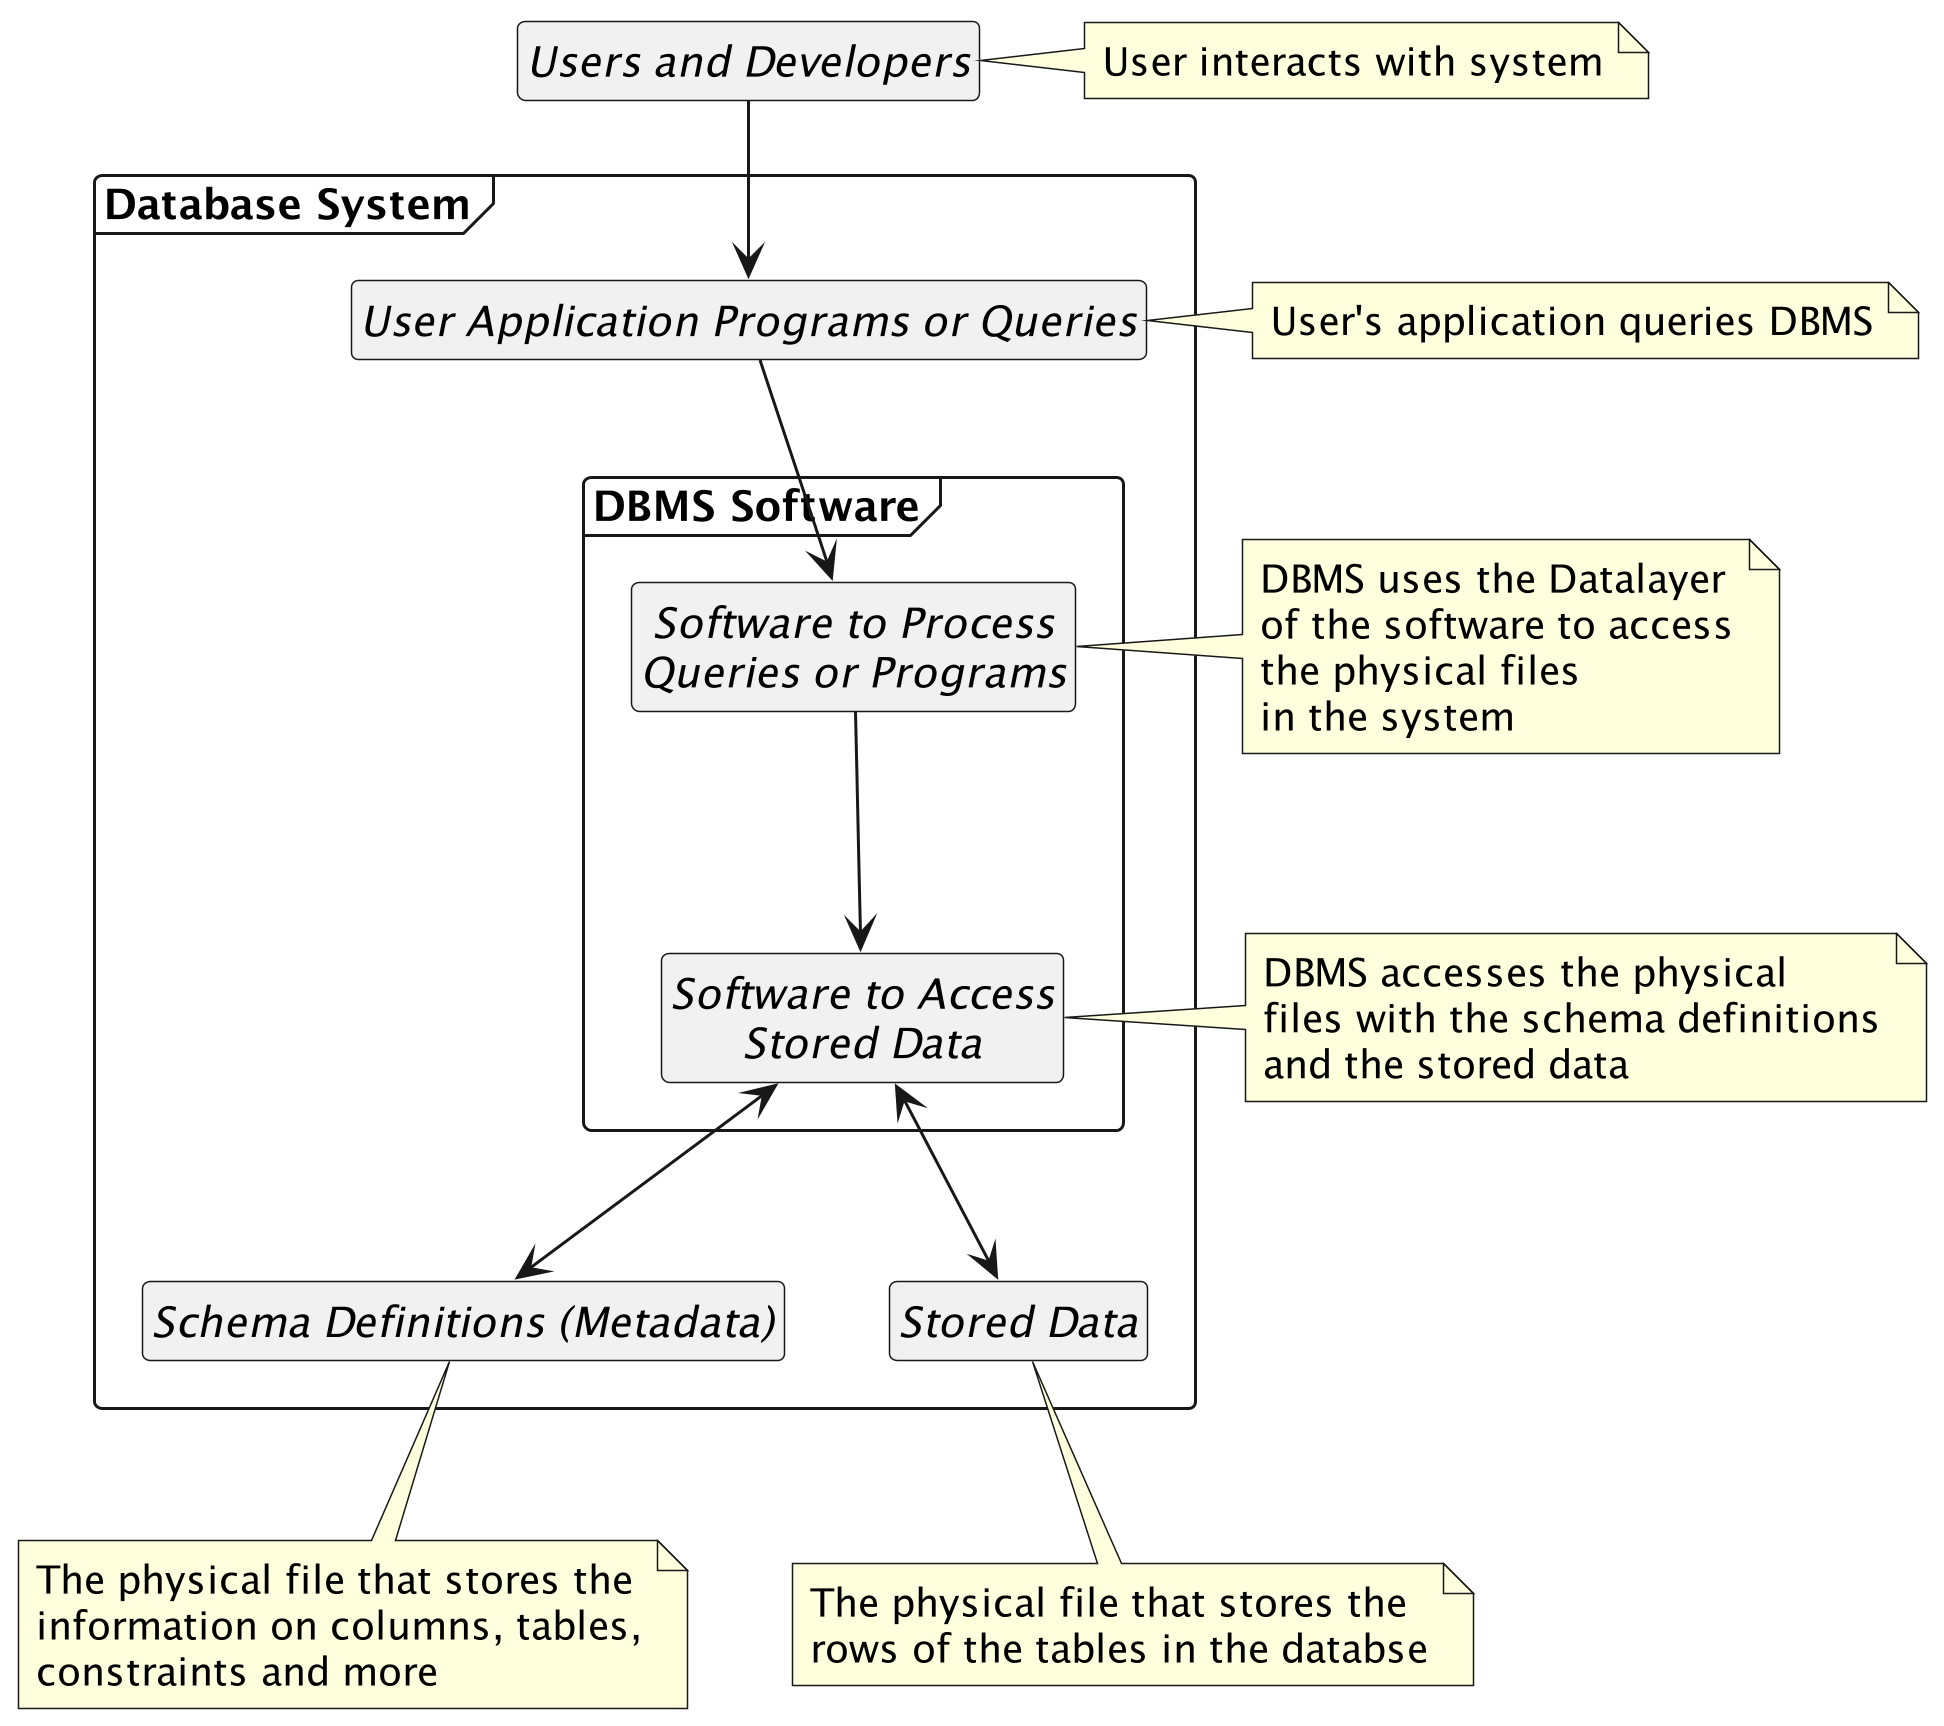
\includegraphics[width=1\textwidth]{content/1-relational-databases/figures/1.dbms-definitions.png}
    \caption{High Level Explanation of a Database Management System}
    \label{fig:1.dbms-definitions.png}
\end{figure}

The relationship among these components is hierarchical and interdependent. At the base, we have the \textbf{Stored Data}, which is the essence of the database. This data is structured and organized according to the \textbf{Schema Definitions}. The \textbf{DBMS Software} serves as the mediator between the stored data and the end-users. It uses the schema definitions to ensure data is correctly stored and retrieved. \textbf{User Application Programs or Queries} interact with the DBMS software to perform operations on the data — whether it's querying for specific information, updating records, or performing analyses. All these components together constitute the \textbf{Database System}, which is the overall environment enabling data management and utilization.

\subsection{The anatomy of a table}
As can be seen in \cref{fig:2.table-definitions.png}, a table is structured through a series of rows and columns that intersect to form cells. Each column in the table is headed by an attribute, which is also commonly referred to as a field, column, or property. These attributes represent the data categories within the table, defining the kind of data each column holds. Similarly, each row in the table is known as a tuple, which can alternatively be called a row, record or an entry. Tuples are instances of the data, encompassing a unique set of values for the attributes defined by the columns. Together, attributes and tuples constitute the fundamental framework of a table.

\begin{figure}[htbp]
    \centering
    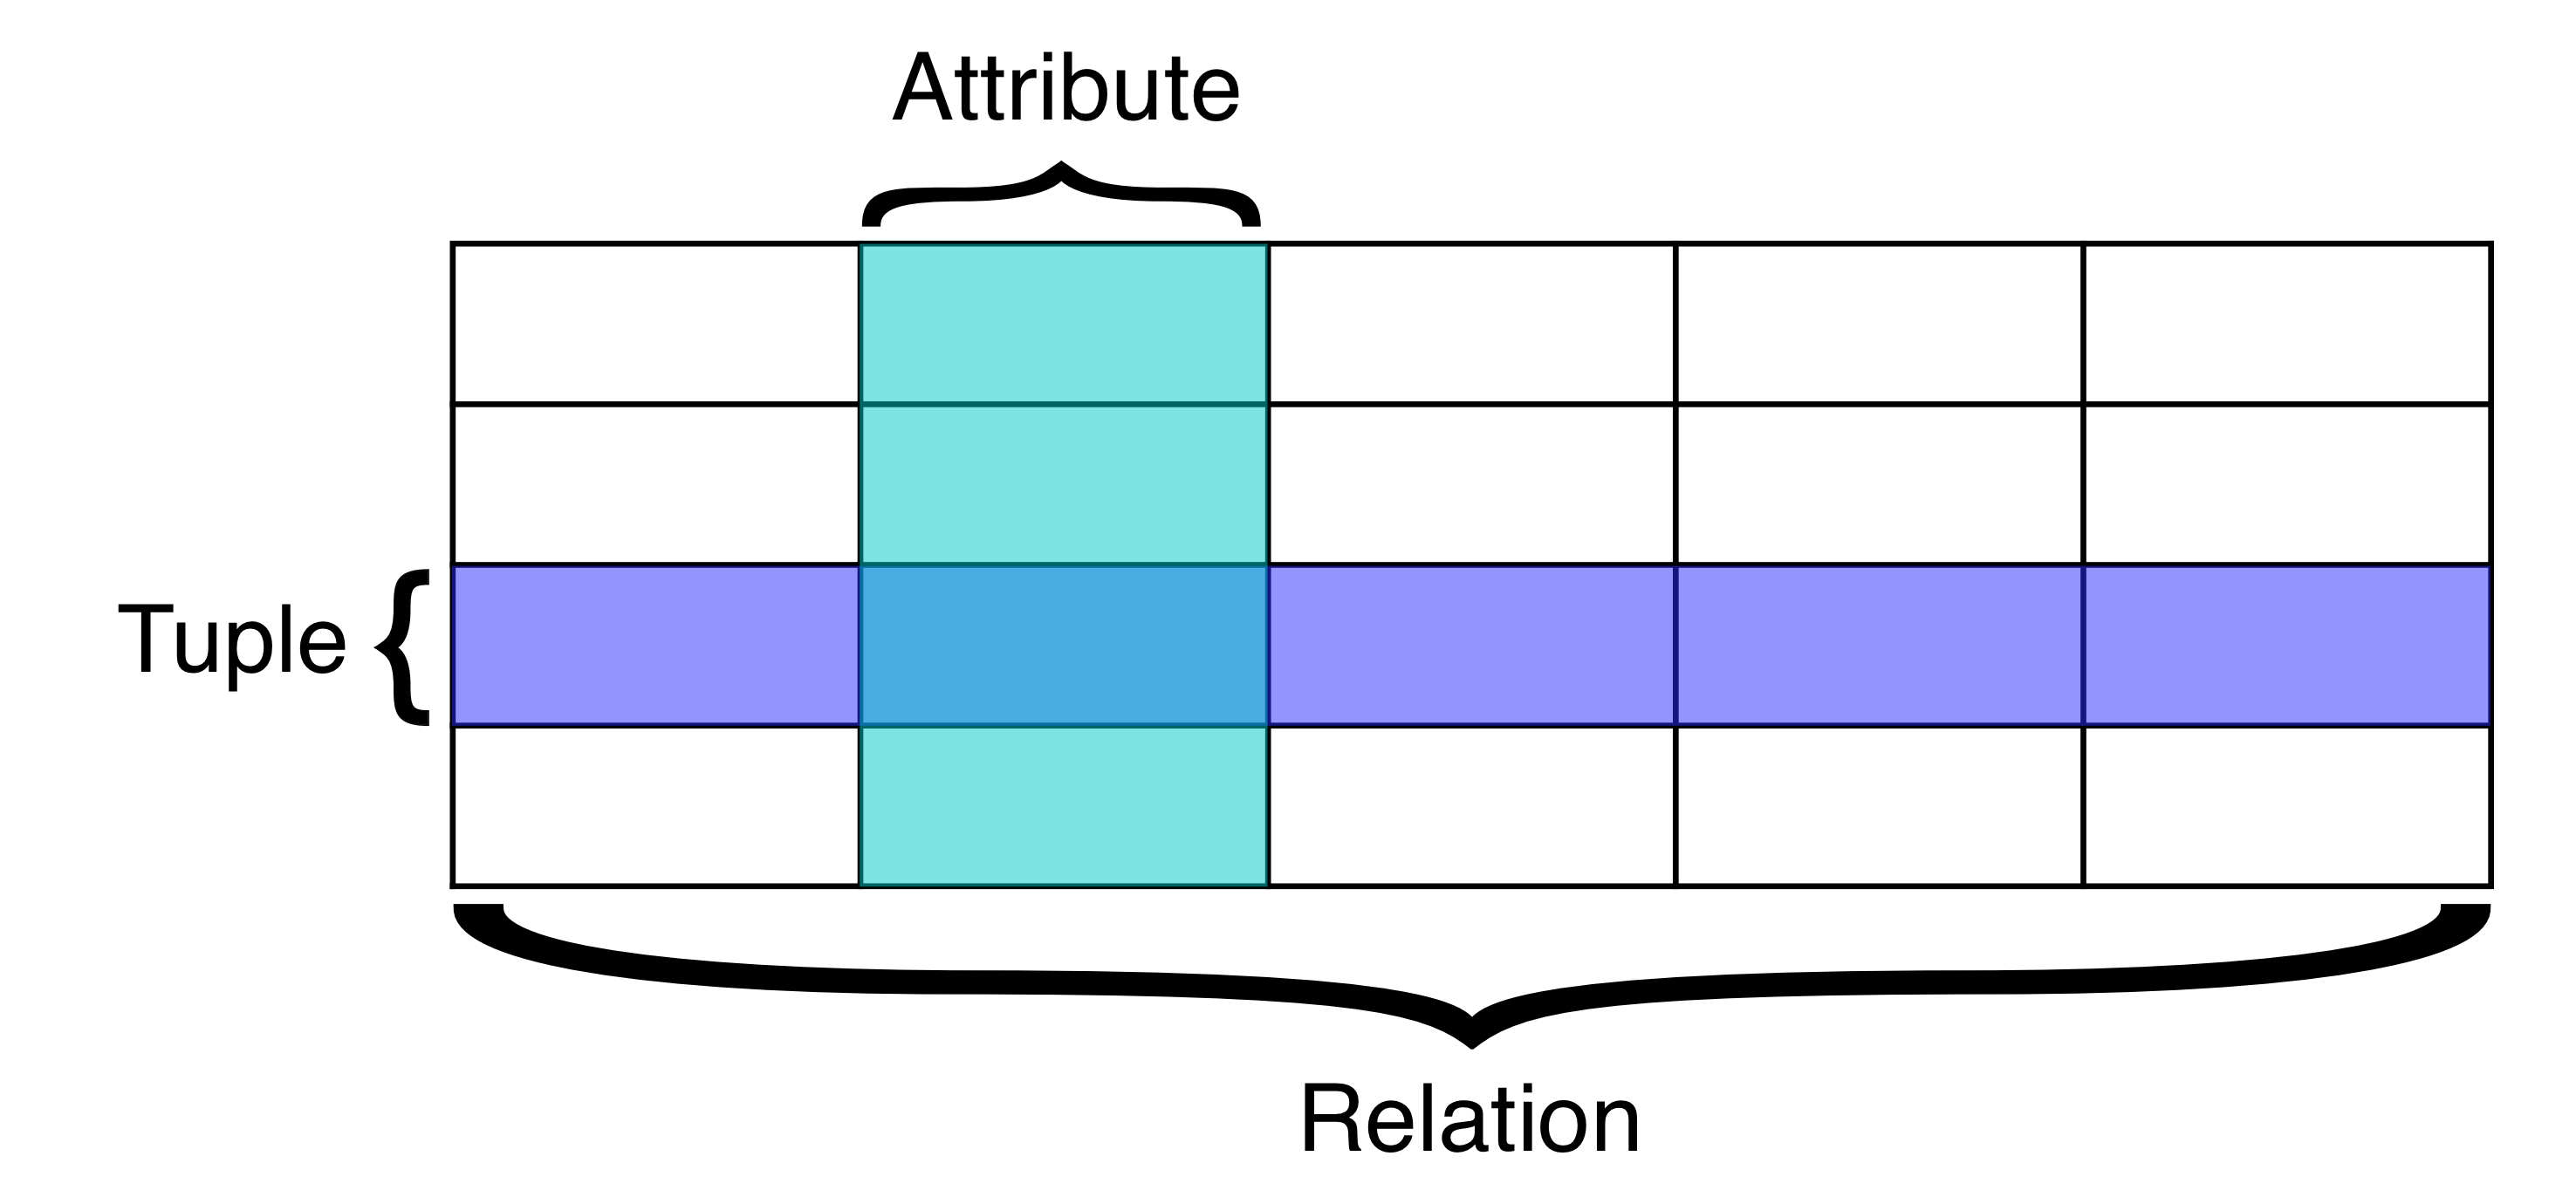
\includegraphics[width=1\textwidth]{content/1-relational-databases/figures/2.table-definitions.png}
    \caption{Table Terminology (Artist: Chris Martin)}
    \label{fig:2.table-definitions.png}
\end{figure}

\section{Setting up your machine}
Before you can start working with databases, you need to set up your machine. This section will guide you through the process of setting up your machine, and installing the required software.

\subsubsection*{Windows Specific Instructions}
Go to https://www.enterprisedb.com/downloads/postgres-postgresql-downloads and download the latest version of PostgreSQL. 
\begin{figure}[htb]
    \centering
    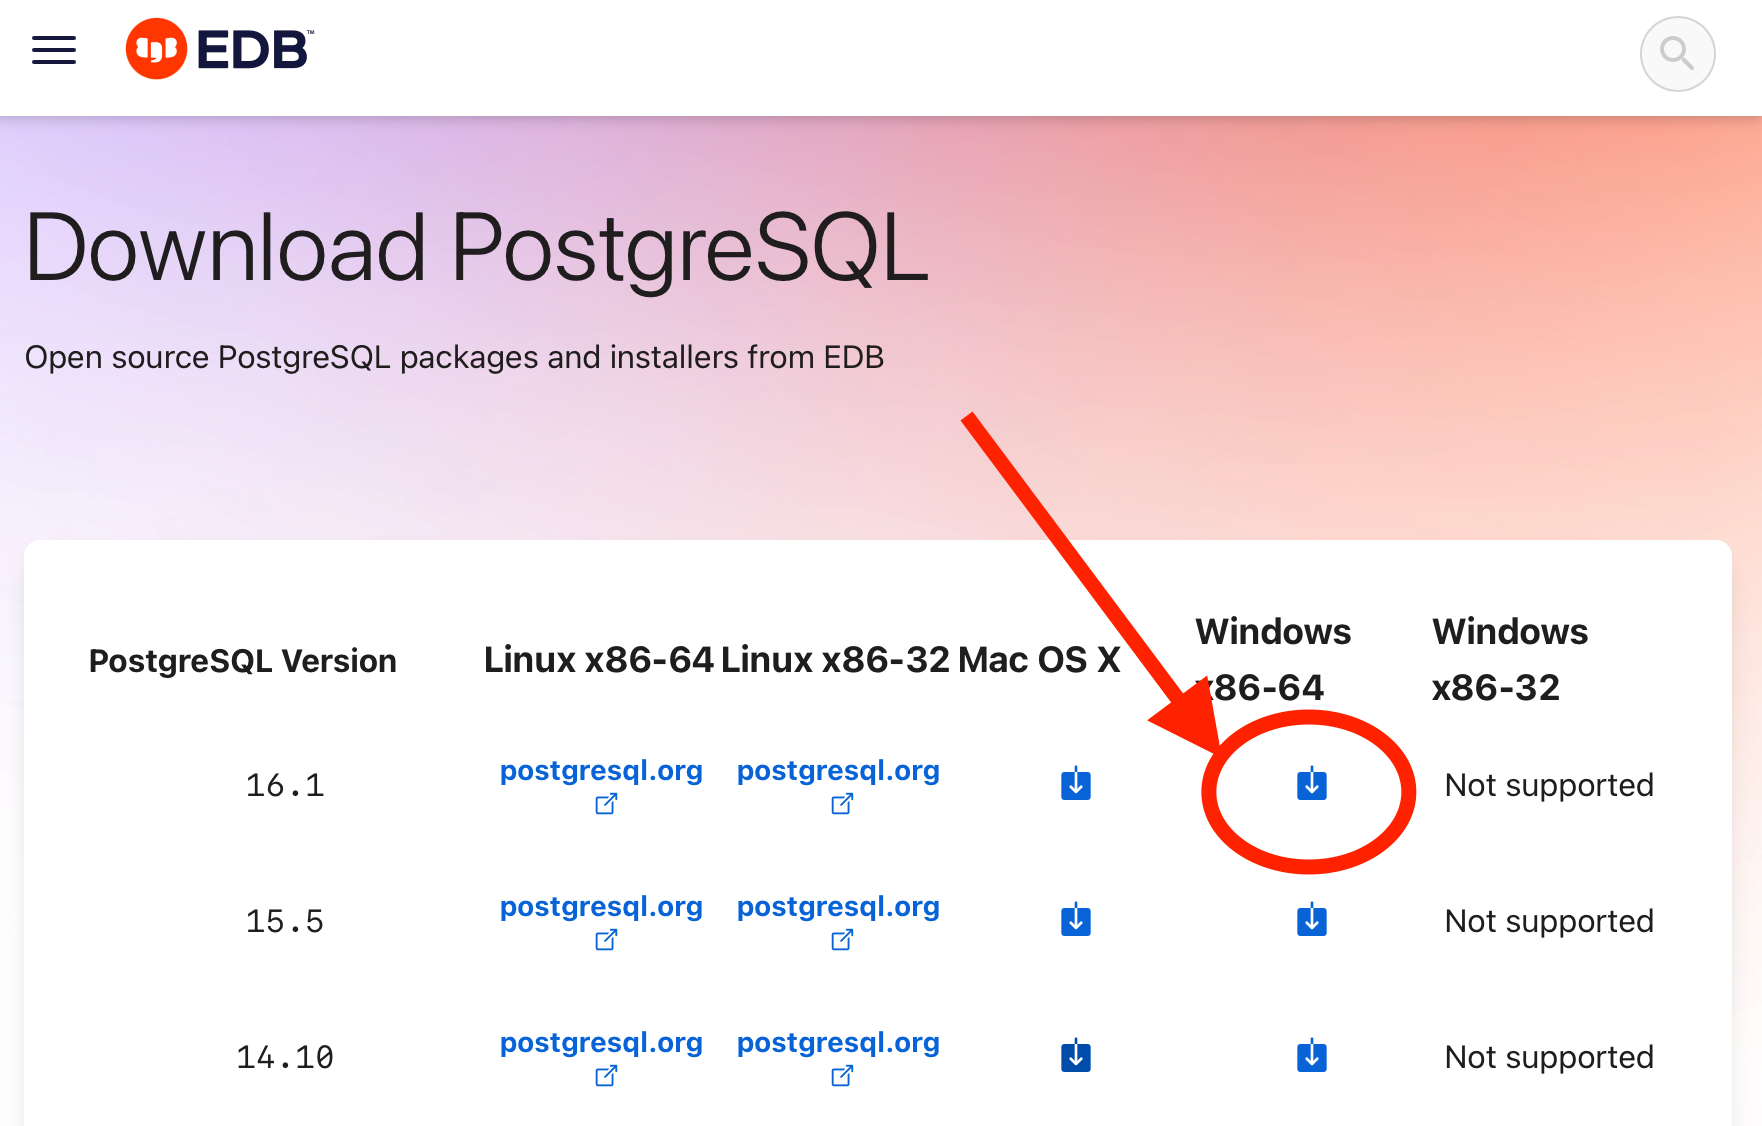
\includegraphics[width=1\textwidth]{content/1-relational-databases/figures/1.install-for-windows-1.png}
    \caption{Download location for PostgreSQL}
    \label{fig:1.postgresql-download-1.png}
\end{figure}

Run the installer, and follow the instructions, but be sure to deselect "Stack Builder" (see \cref{fig:1.postgresql-download-2.png}), as we will not be using it in this book. 

\begin{figure}[htb]
    \centering
    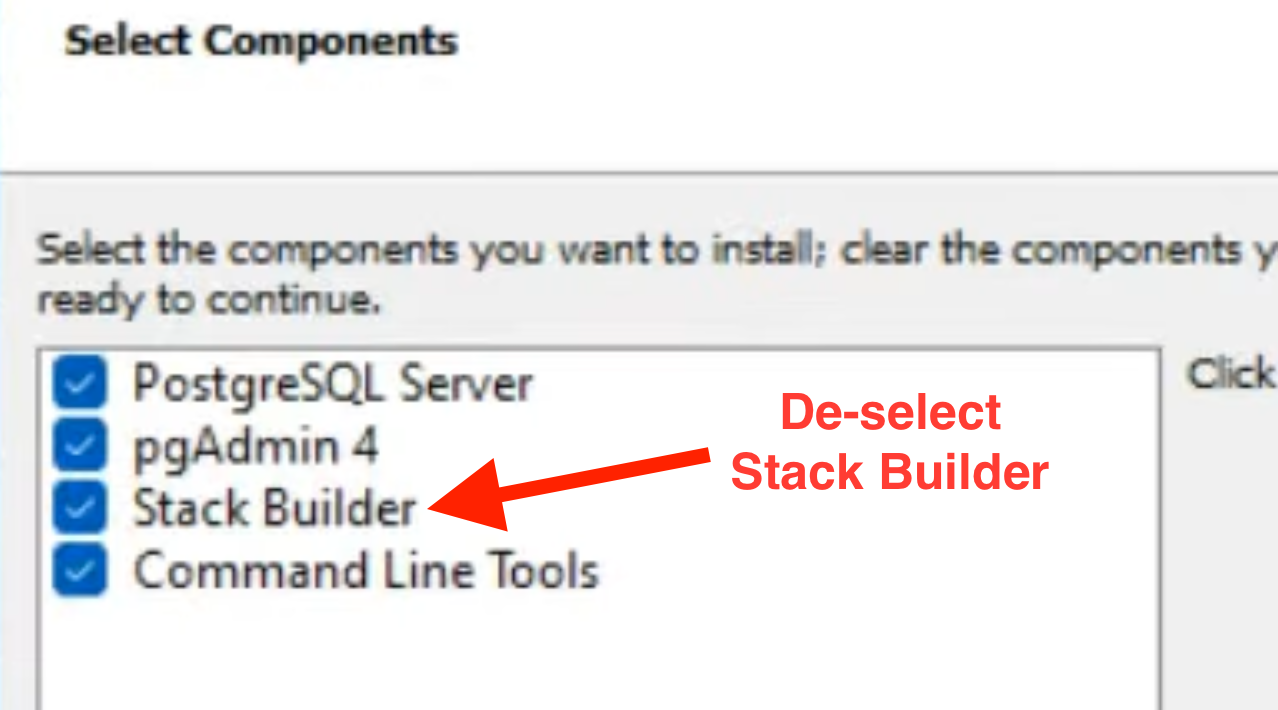
\includegraphics[width=0.6\textwidth]{content/1-relational-databases/figures/1.install-for-windows-2.png}
    \caption{Components to install}
    \label{fig:1.postgresql-download-2.png}
\end{figure}

When asked for a password, use the password you want to use for the postgres user. This is the user that is used to manage the database server. Be sure to remember this password, as you will need it later. After this password it set, the database server instance will have the user postgres, and the password will be what you set. Beware that your computers password, the database server instance password, and the pgAdmin password are all different passwords.

\begin{figure}[htb]
    \centering
    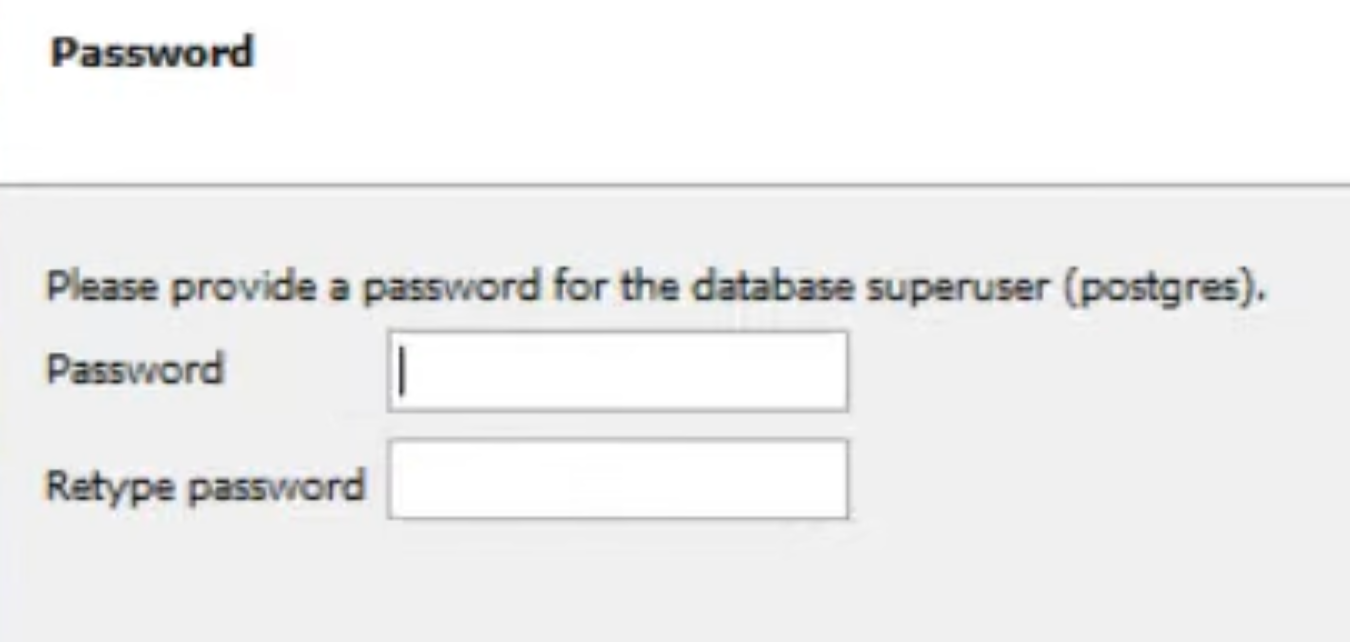
\includegraphics[width=0.7\textwidth]{content/1-relational-databases/figures/1.install-for-windows-3.png}
    \caption{Pick a password for the postgres user}
    \label{fig:1.postgresql-download-3.png}
\end{figure}


This is not the password you will use to connect to the database server, but the password you will use to manage the database server. This password is not used in this book, but it is good practice to set it to something you can remember.

\subsubsection*{Mac Specific Instructions}
Installation of PostgreSQL on a Mac is done through the terminal. You can pick any way to do this, but we are going to use the homebrew (https://brew.sh) solution. Open the terminal, and run the following command to install homebrew: 

\begin{minted}[fontsize=\footnotesize]{bash}
    /bin/bash -c "$(curl -fsSL https://raw.githubusercontent.com
        /Homebrew/install/HEAD/install.sh)"
\end{minted}

Or copy it directly from the frontpage of the homebrew website. After homebrew is installed, you can install PostgreSQL by running the following command in the terminal:

\begin{minted}[fontsize=\footnotesize]{bash}
    brew install postgresql
    /opt/homebrew/bin/createuser -s postgres
\end{minted}

After PostgreSQL is installed, you can start the server by running the following command in the terminal:

\begin{minted}[fontsize=\footnotesize]{bash}
    brew services start postgresql
\end{minted}

This will start the PostgreSQL server, and it will start automatically every time you start your computer. If you want to stop the server, you can run the following command in the terminal:

\begin{minted}[fontsize=\footnotesize]{bash}
    brew services stop postgresql
\end{minted}

And if you only want to start the server once, you can run the following command in the terminal:

\begin{minted}[fontsize=\footnotesize]{bash}
    brew services run postgresql
\end{minted}


PostgreSQL will not have a password set at this point, and a password needs to be set using the comandline. It can be set by running the following command in the terminal:

\begin{minted}[fontsize=\footnotesize]{bash}
    psql postgres
    \password postgres
\end{minted}

Running the above code will prompt you to write a password for the postgres user. Remember this password, as you will need it every time you connect to the database server instance. 


Remember to also install pgAdmin using homebrew, by running the following command in the terminal:
\begin{minted}[fontsize=\footnotesize]{bash}
    brew install pgadmin4
\end{minted}

At the first run of pgadmin a password needs to be set. Remember it, as you need it every time you used pgadmin. Be aware that this password is not the same as the password for the database server instance, and the password for the postgres user.


\subsubsection*{Linux Specific Instructions}
With linux, you are mostly on your own, but generally, most linux distributions have a package manager that you can use to install PostgreSQL. The package manager is different from distribution to distribution, but the most common ones are apt, yum, and dnf. To install PostgreSQL on Ubuntu, you can run the following command in the terminal:

\begin{minted}[fontsize=\footnotesize]{bash}
    sudo apt-get install postgresql
\end{minted}

After PostgreSQL is installed, you can start the server by running the following command in the terminal:

\begin{minted}[fontsize=\footnotesize]{bash}
    sudo systemctl start postgresql
\end{minted}

This will start the PostgreSQL server, and it will start automatically every time you start your computer. If you want to stop the server, you can run the following command in the terminal:

\begin{minted}[fontsize=\footnotesize]{bash}
    sudo systemctl stop postgresql
\end{minted}

PostgreSQL will not have a password set at this point, and a password needs to be set using the comandline. It can be set by running the following command in the terminal:

\begin{minted}[fontsize=\footnotesize]{bash}
    psql postgres
    \password postgres
\end{minted}

Running the above code will prompt you to write a password for the postgres user. Remember this password, as you will need it every time you connect to the database server instance. 

Remember to install pgAdmin too. This can be done using the package manager of your distribution. With Ubuntu, you can run the following command in the terminal:

\begin{minted}[fontsize=\footnotesize]{bash}
    sudo apt-get install pgadmin4
\end{minted}

At the first run of pgadmin a password needs to be set. Remember it, as you need it every time you used pgadmin. Be aware that this password is not the same as the password for the database server instance, and the password for the postgres user.

\section{Connecting to the database with pgAdmin}
When you have installed PostgreSQL, you can connect to the database using pgAdmin. pgAdmin is a graphical user interface that allows you to interact with the database. It is a powerful tool that allows you to create, manage, and query databases. This section will guide you through the process of connecting to the database using pgAdmin.

First start the application in your respective operating system. The application will look like \cref{fig:1.pgadmin1}.
\begin{figure}[H]
    \centering
    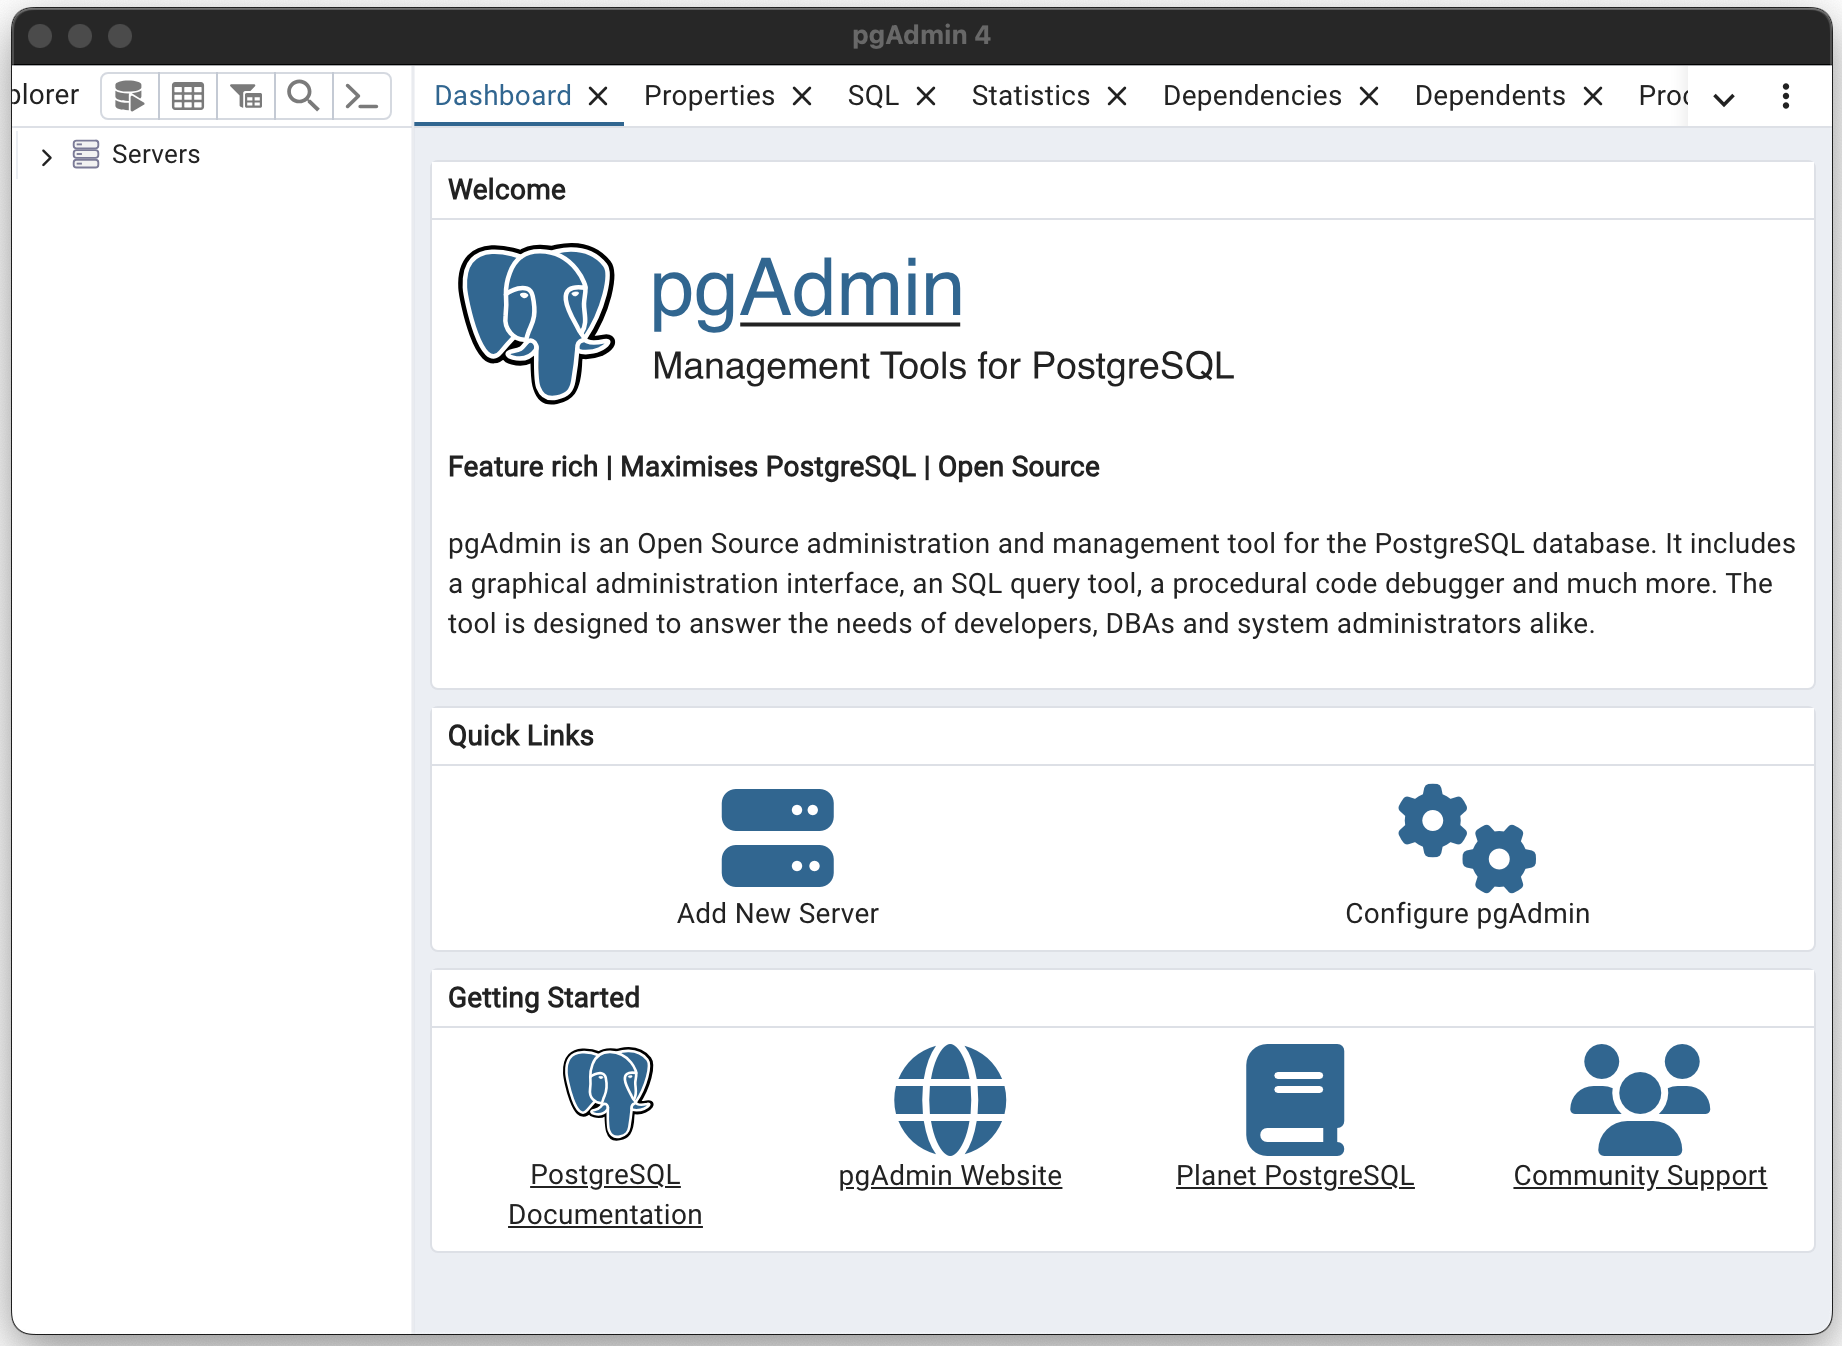
\includegraphics[width=0.7\textwidth]{content/1-relational-databases/figures/pgadmin/1.png}
    \caption{Starting pgAdmin}
    \label{fig:1.pgadmin1}
\end{figure}

Next, you need to register a server. This is done by right clicking on the "Servers" node in the tree view, and selecting "Create" and then "Server...". This will open a dialog where you can fill in the connection information. The dialog will look like \cref{fig:1.pgadmin2}.

\begin{figure}[H]
    \centering
    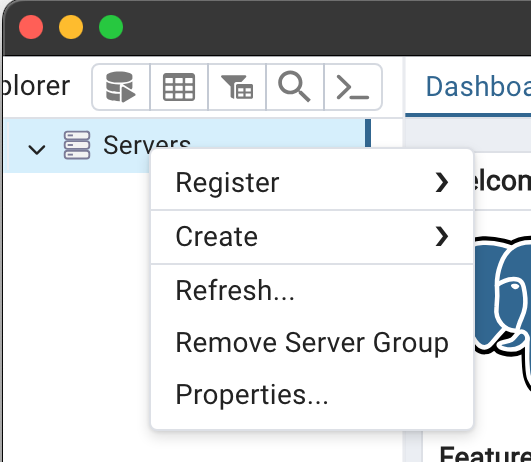
\includegraphics[width=0.3\textwidth]{content/1-relational-databases/figures/pgadmin/2.png}
    \caption{Initiate registration of a server}
    \label{fig:1.pgadmin2}
\end{figure}


% The dialog will look like \cref{fig:1.pgadmin3}.

% \begin{figure}[H]
%     \centering
%     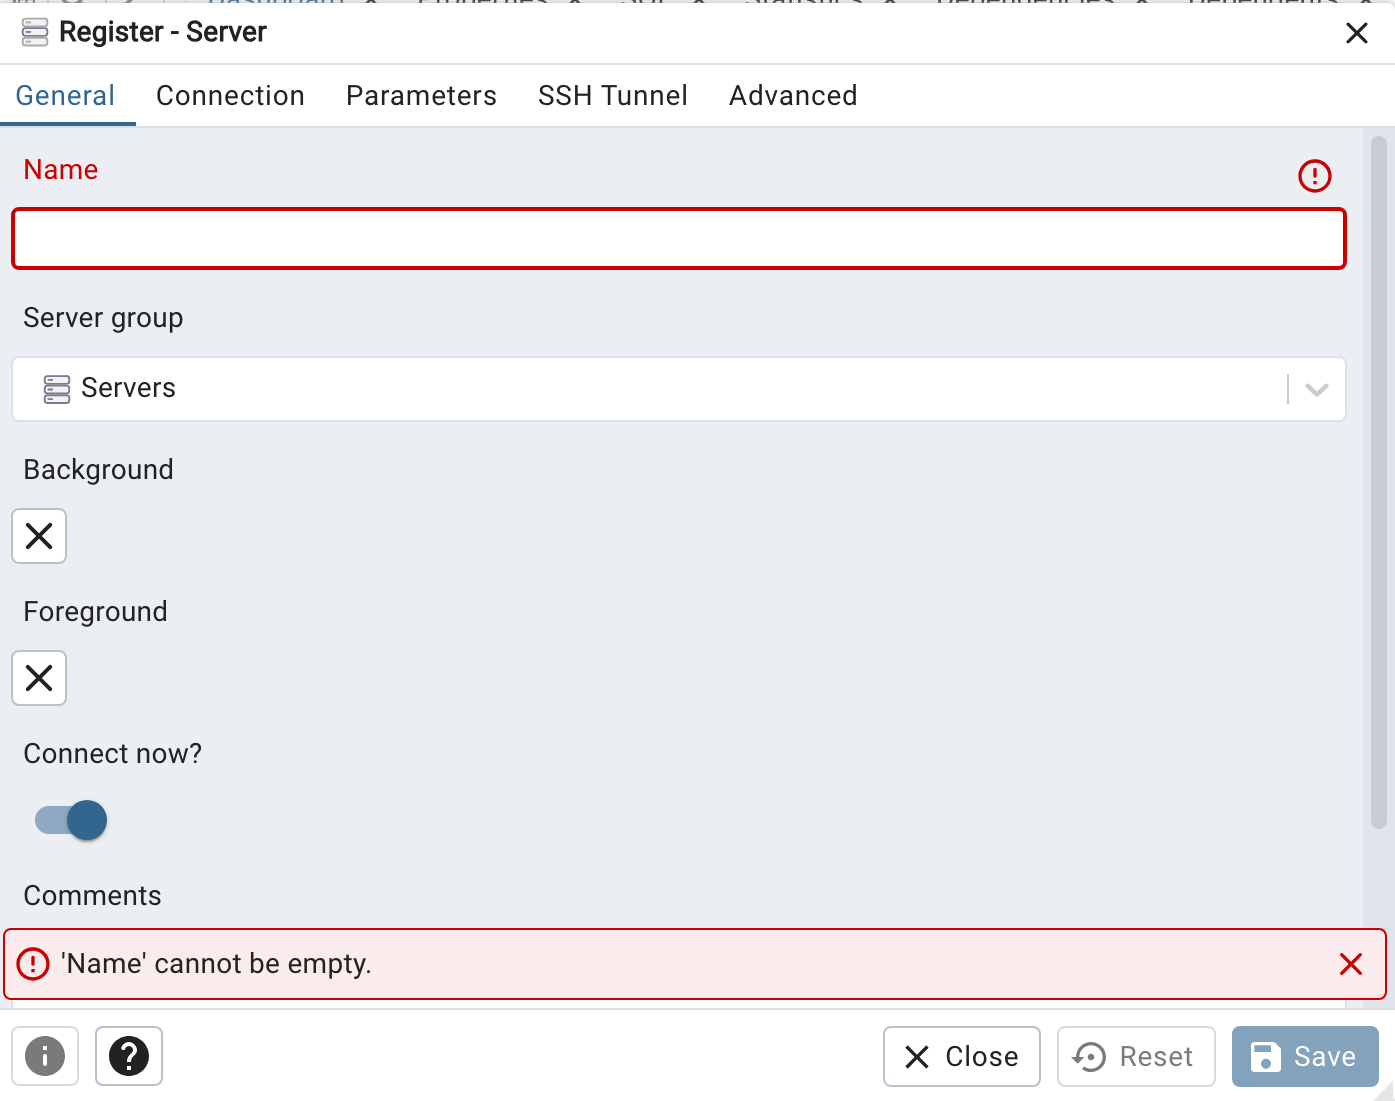
\includegraphics[width=0.6\textwidth]{content/1-relational-databases/figures/pgadmin/3.png}
%     \caption{Pick a name, i recommend localhost}
%     \label{fig:1.pgadmin3}
% \end{figure}

Pick a name for the server, and click save. I recommend localhost, as it is the default name, and as it refers to your local computer. This is convention for development machines. 
Move to the tab "Connection", and fill in the connection information. The hostname is localhost, the username is postgres, and the password is the password you set for the postgres user. The dialog will look like \cref{fig:1.pgadmin4}.

\begin{figure}[H]
    \centering
    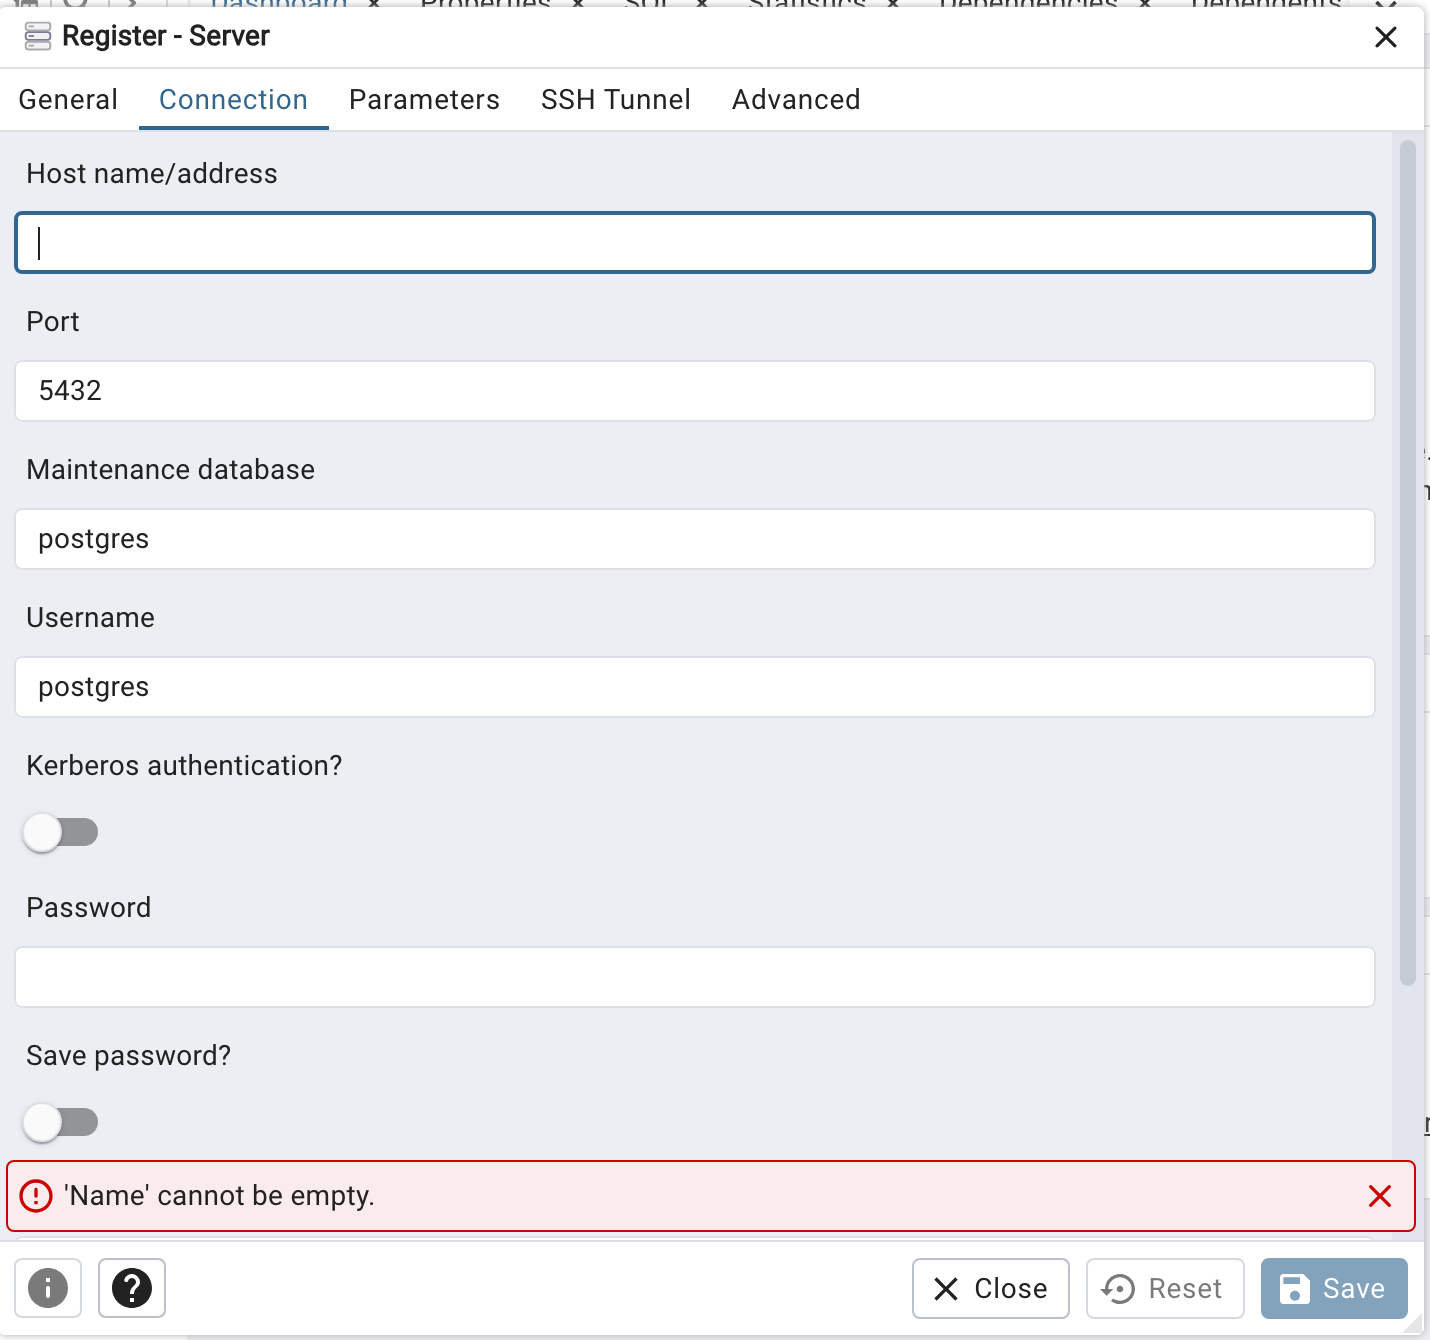
\includegraphics[width=0.6\textwidth]{content/1-relational-databases/figures/pgadmin/4.png}
    \caption{Fill in connection information, hostname is localhost, username is postgres, and the password is the password you set for the postgres user}
    \label{fig:1.pgadmin4}
\end{figure}

% If you have filled in the information correctly, you will see a success message like \cref{fig:1.pgadmin5}. If you see this message, you have successfully connected to the database server instance.

% \begin{figure}[h]
%     \centering
%     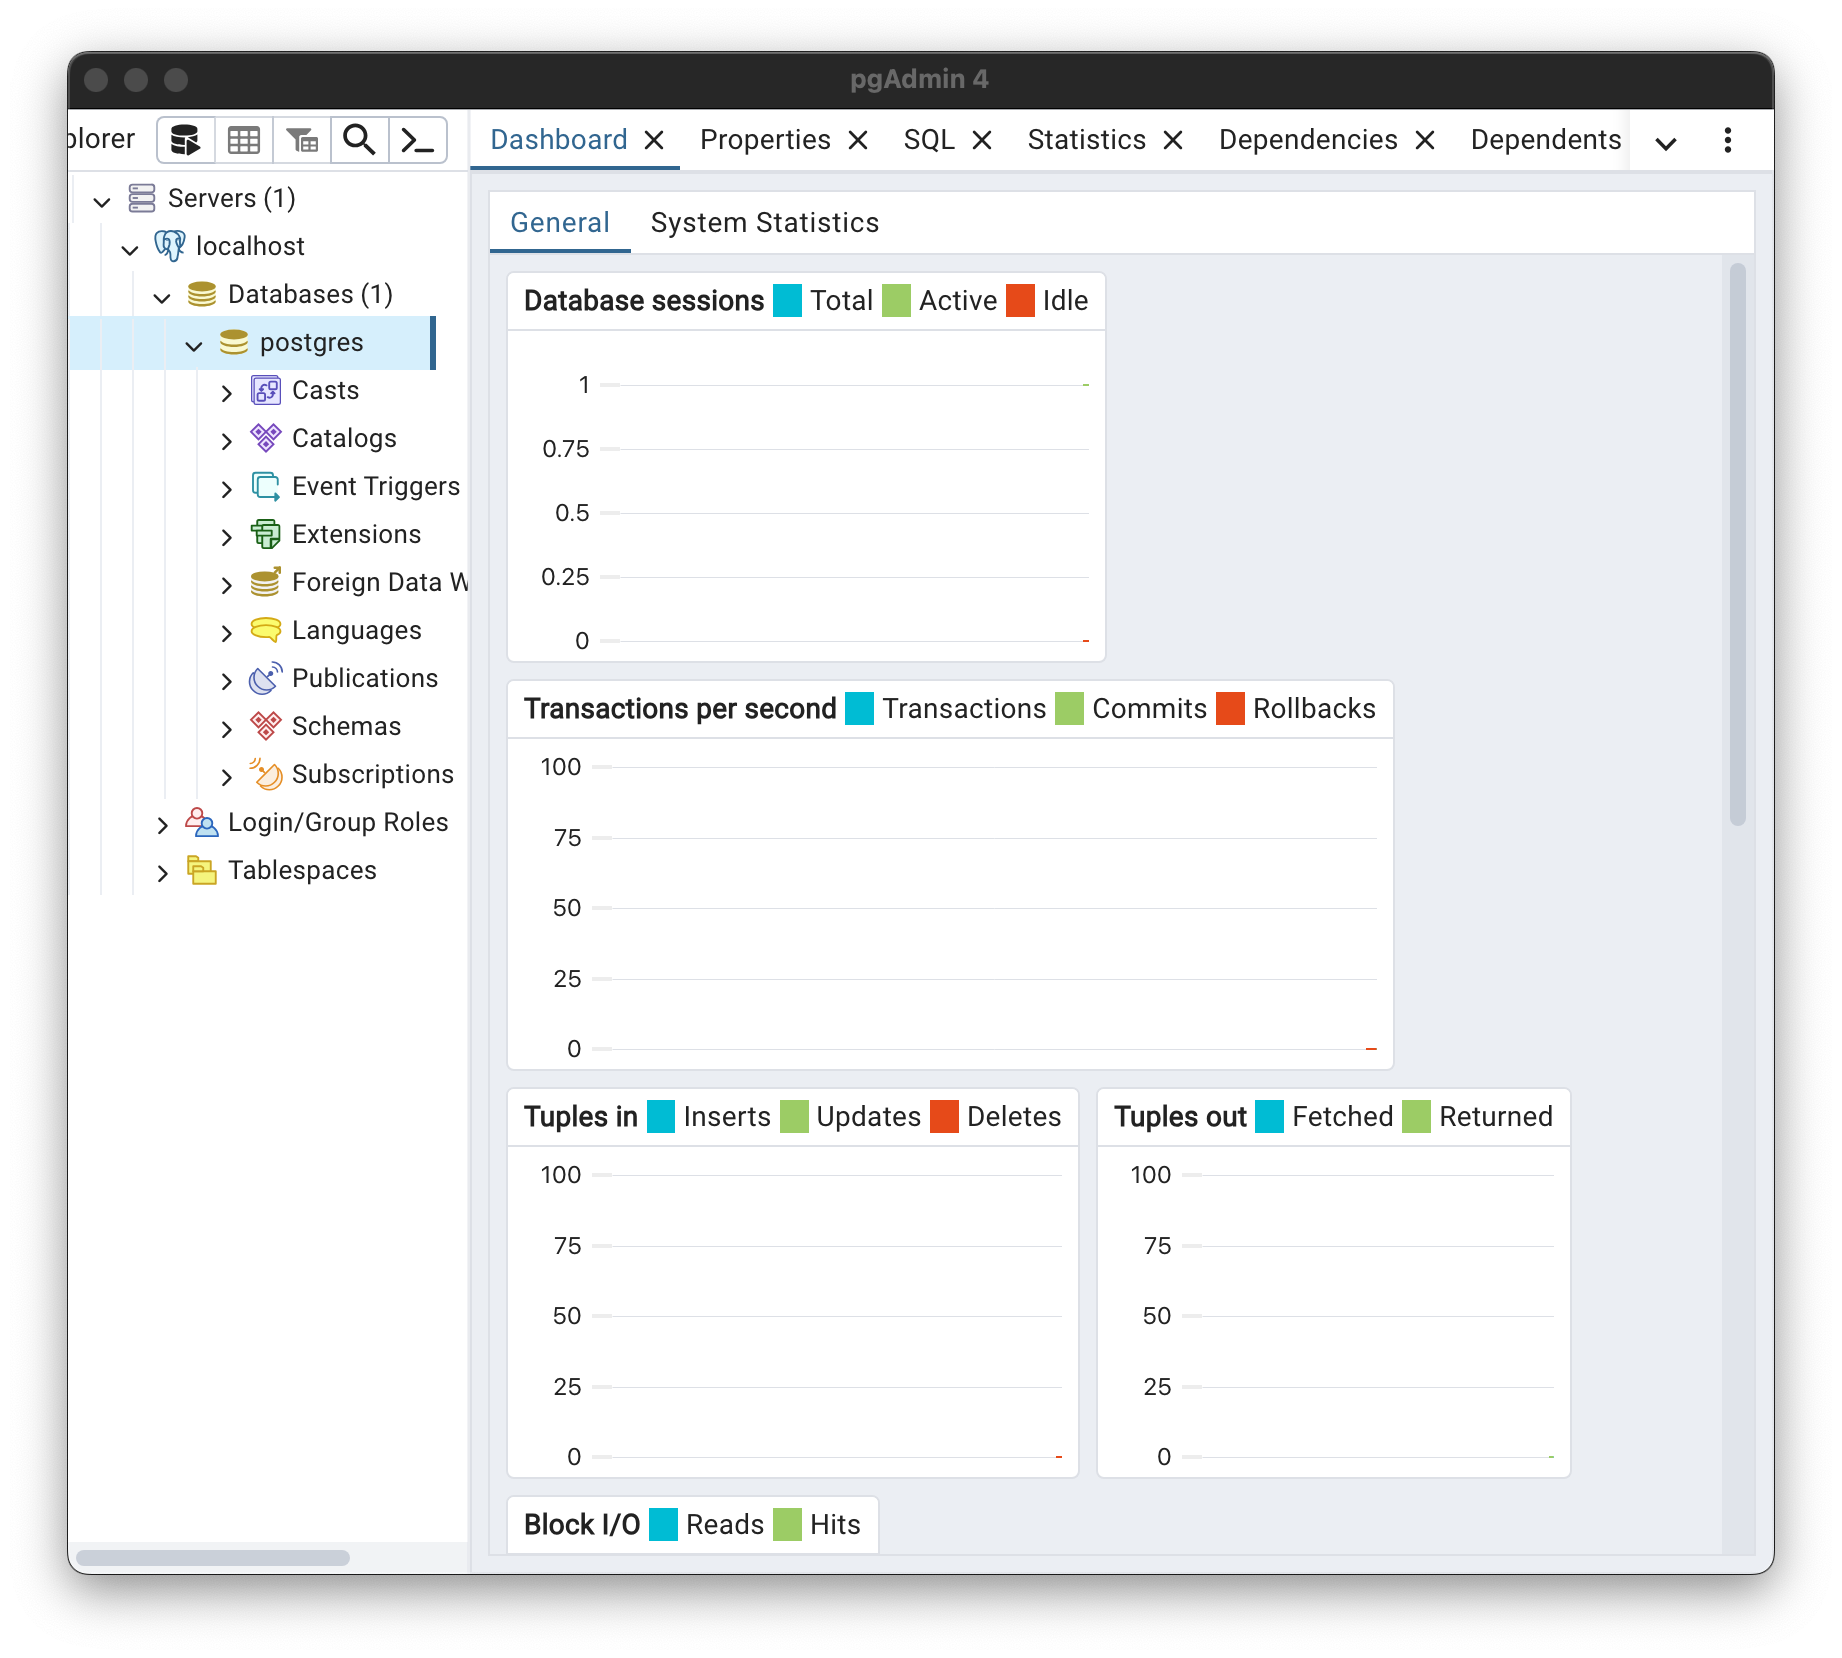
\includegraphics[width=0.7\textwidth]{content/1-relational-databases/figures/pgadmin/5.png}
%     \caption{Success looks like this!}
%     \label{fig:1.pgadmin5}
% \end{figure}
You should now be connected to the database and see it in the right pane.
Now you can create a new database. This is done by right clicking on the "Databases" node in the tree view, and selecting "Create" and then "Database...". This will open a dialog where you can fill in the database information. The dialog will look like \cref{fig:1.pgadmin6}.

\begin{figure}[H]
    \centering
    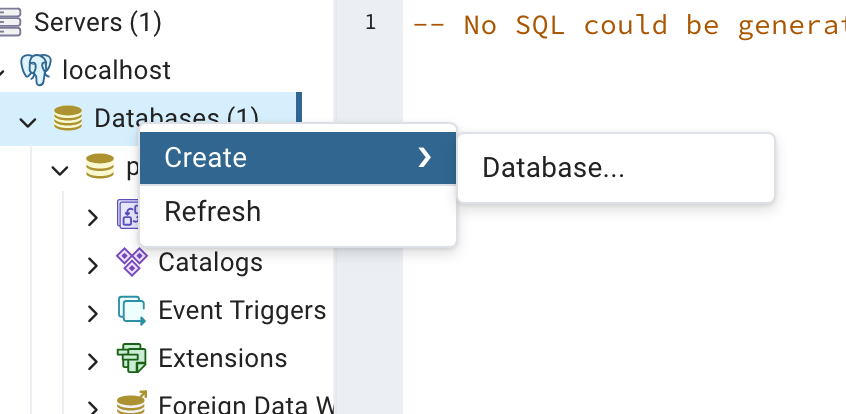
\includegraphics[width=0.5\textwidth]{content/1-relational-databases/figures/pgadmin/6.png}
    \caption{Creating a new database from pgAdmin}
    \label{fig:1.pgadmin6}
\end{figure}

Pick a name for the database, and click save. The dialog will look like \cref{fig:1.pgadmin7}.

\begin{figure}[H]
    \centering
    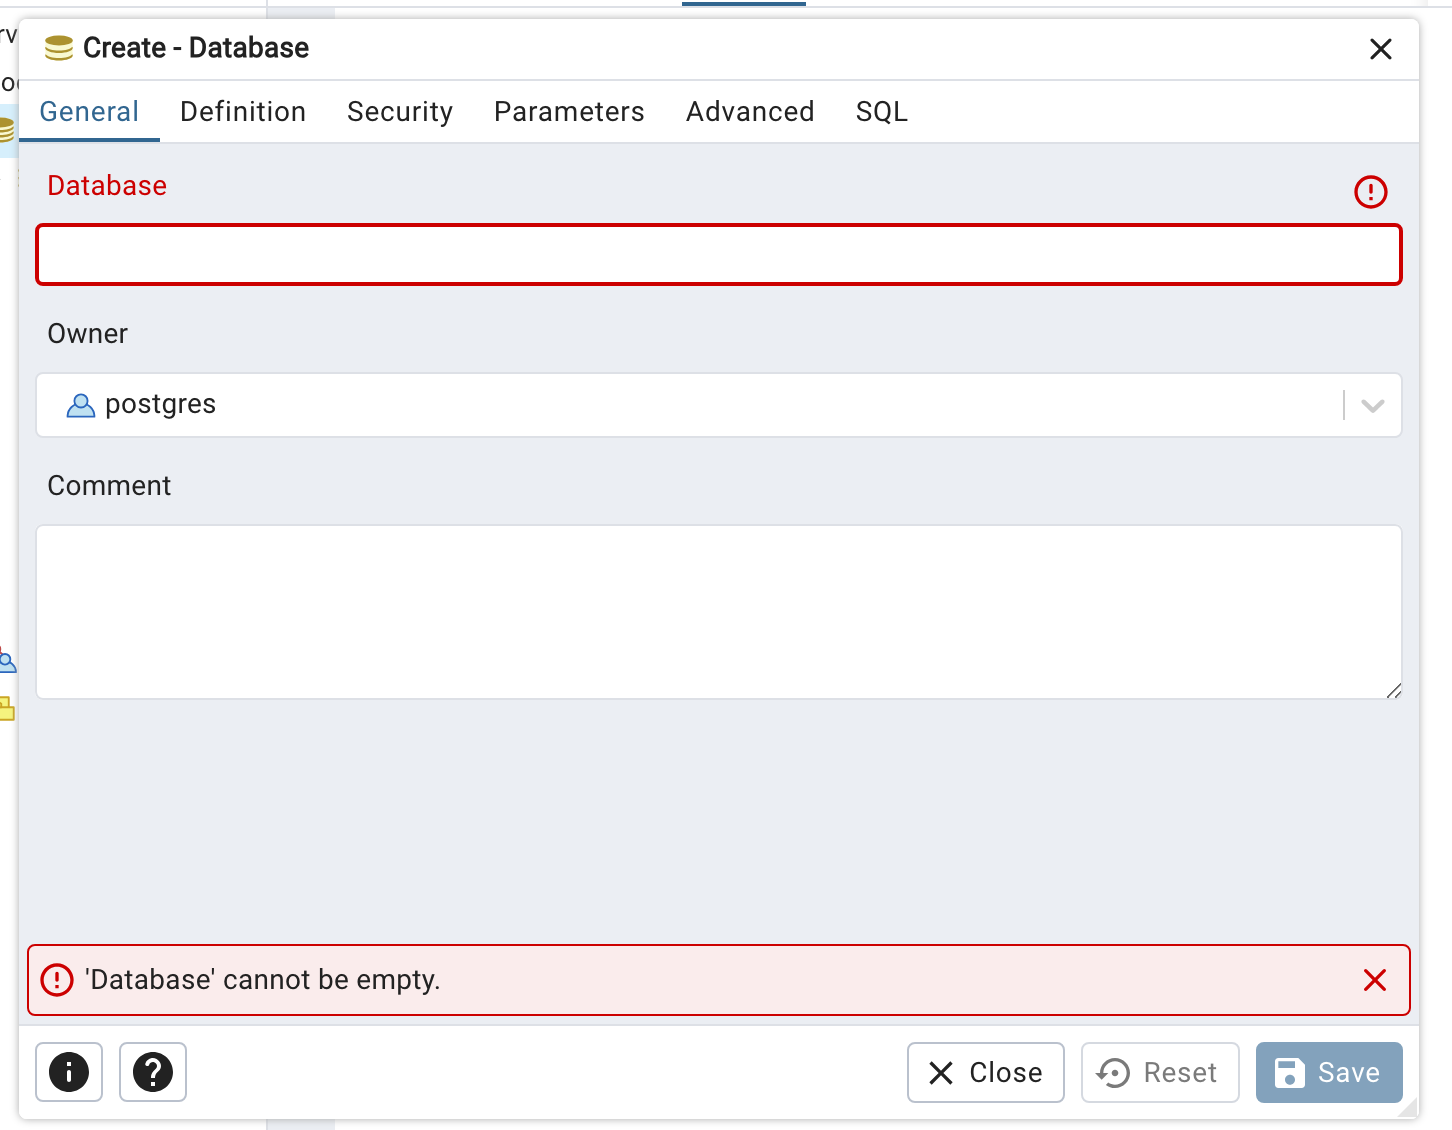
\includegraphics[width=0.7\textwidth]{content/1-relational-databases/figures/pgadmin/7.png}
    \caption{Pick a database name, and click save}
    \label{fig:1.pgadmin7}
\end{figure}

Now you have created a database, and you can start working with it. You can start by creating tables, and inserting data into the tables. This is done by right clicking on the database, and selecting "Query Tool". This will open a dialog where you can write your code, and execute it. The dialog will look like \cref{fig:1.pgadmin8}.

\begin{figure}[H]
    \centering
    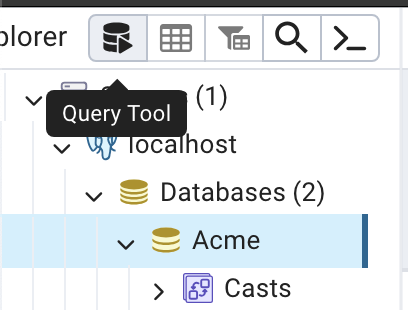
\includegraphics[width=0.4\textwidth]{content/1-relational-databases/figures/pgadmin/8.png}
    \caption{Mark the database, and press the query tool}
    \label{fig:1.pgadmin8}
\end{figure}

Write your code, and execute it. The dialog will look like \cref{fig:1.pgadmin9}. You are now ready for coding.

\begin{figure}[H]
    \centering
    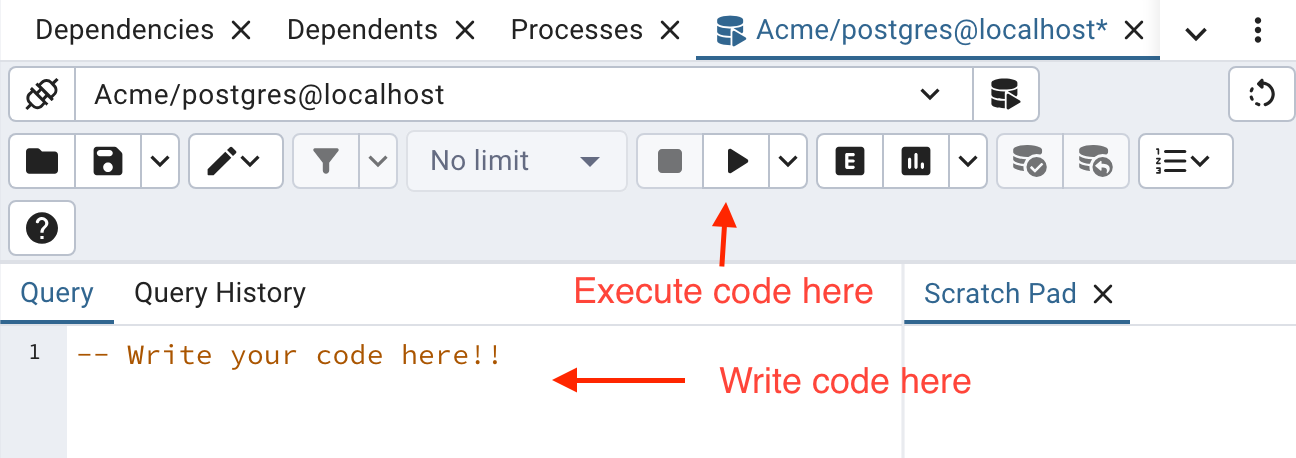
\includegraphics[width=0.7\textwidth]{content/1-relational-databases/figures/pgadmin/9.png}
    \caption{Write your code, and execute it}
    \label{fig:1.pgadmin9}
\end{figure}

Now that your machine is ready, and you have connected to the database, you are ready to start working with databases. The next chapter will guide you through the process of creating a database, and managing tables, as well as how to query the database.


% ******************************* Chapter: Relational Database Basics ****************************
\chapter{Relational Database Basics}
\label{chap:relational:relational-database-basics}
This chapter contains the basic building blocks to get started with basic relational databases.
It will explain the basic concepts of databases, and how to create, manage, and query a database.

\section{Creating your first database}
Creating a database is the first step in working with databases. This section will guide you through the process of creating a database. 

The following codesnippet shows the available syntax for the create database operation. The syntax is the same for all database management systems, but the options available might differ. The options available in PostgreSQL are shown in the example.

\begin{minted}[fontsize=\footnotesize]{postgresql}
    -- Creating a database with full syntax
    CREATE DATABASE database_name
    WITH
        [OWNER =  role_name]
        [TEMPLATE = template]
        [ENCODING = encoding]
        [LC_COLLATE = collate]
        [LC_CTYPE = ctype]
        [TABLESPACE = tablespace_name]
        [ALLOW_CONNECTIONS = true | false]
        [CONNECTION LIMIT = max_concurrent_connection]
        [IS_TEMPLATE = true | false ]
\end{minted}

The key element to understand here is that the name of the CREATE DATABASE statement and a database name of your choosing is mandatory, the WITH clause and everything after it is optional. If no parameters are set, the database will be created with default settings. Therefore, the simplest way to create a database is to run the following command:

\begin{minted}[fontsize=\footnotesize]{postgresql}
    -- Creating an ACME database with minimal syntax
    CREATE DATABASE Acme;
\end{minted}

Note that both examples you have seen until now, are also using comments. A double dash "--" creates a one-line comment, and a slash-star "/*" creates a multi-line comment. Comments are not executed, and are only there to help you understand the code. It does, however, make the code more readable and understandable, and is therefore a good practice to use comments.

If you wish to create a database with specific settings, you can use the WITH clause. The following example shows how to create a database with specific settings:

\begin{minted}[fontsize=\footnotesize]{postgresql}
    -- Creating a ACME database with enabled options
    CREATE DATABASE Acme 
    WITH
        OWNER = postgres
        CONNECTION LIMIT = 50;
        IS_TEMPLATE = false;
\end{minted}

\subsection{Altering and deleting databases}
If you wish an already existing database settings can be altered. The following example shows how to alter a database, and disable index scans (which is not recommended):

\begin{minted}[fontsize=\footnotesize]{postgresql}
    -- Alter Database Acme to disable index scans
    ALTER DATABASE Acme SET enable_indexscan TO off;
\end{minted}

The last missing component is how to delete a database. The following example shows how to delete a database. Beware that this is a permanent operation, and that all data in the database will be lost with no way to recover the data!

\begin{minted}[fontsize=\footnotesize]{postgresql}
    -- Delete a table
    DROP DATABASE Acme;
\end{minted}

\subsection{Switch databases}
It is also possible to switch between databases within the same script on most database management systems. Inside the script, one can freely change databases and run queries on different databases. The following example shows how to switch databases in in Microsoft SQL:

\begin{minted}[fontsize=\footnotesize]{sql}
    /* Change to database_name
     * This does not work with PostgreSQL */
    USE database_name;
\end{minted}

However, this does not work with PostgreSQL. PostgreSQL is implemented differently, and requires that you actively with your graphical user interface, or with the command line, switch to the database you want to work with. The following example shows how to switch databases in PostgreSQL from the command line using psql:

\begin{minted}[fontsize=\footnotesize]{psql}
    -- Change to database_name from psql command line
    \connect database_name
\end{minted}


\section{Managing Tables}
For the first database to actually hold any data, it needs to have tables. This section will guide you through the process of creating, altering, and deleting tables.

\subsection{Creating tables}
\begin{minted}[fontsize=\footnotesize]{postgresql}
    -- Create a table
    CREATE TABLE tableName (
        tableName_id SERIAL PRIMARY KEY, -- auto incrementing id
        username VARCHAR (50) UNIQUE NOT NULL, -- unique username
        password VARCHAR (250) NOT NULL -- never store in plain text
    );
\end{minted}

\begin{minted}[fontsize=\footnotesize]{postgresql}
    -- Create account table
    CREATE TABLE account (
        id serial PRIMARY KEY,
        username VARCHAR (50) UNIQUE NOT NULL,
        created_on TIMESTAMP NOT NULL, 
        last_login TIMESTAMP
    );
    
    /* Create blog entries table
     * the created_by column references the 
     * id column in the account table */
    CREATE TABLE blog_entries (
        id serial PRIMARY KEY, 
        header VARCHAR (255) NOT NULL,
        body TEXT NOT NULL,
        created_by INTEGER NOT NULL REFERENCES account (id)
    );
\end{minted}

\subsection{Altering tables}
\begin{minted}[fontsize=\footnotesize]{postgresql}
    -- Create a table
    CREATE TABLE account (
        user_id SERIAL PRIMARY KEY,
        username VARCHAR (50) UNIQUE NOT NULL,
        password VARCHAR (50) NOT NULL,
        email VARCHAR (355) UNIQUE NOT NULL,
        created_on TIMESTAMP NOT NULL,
        last_login TIMESTAMP
    );
\end{minted}

\subsection{Deleting tables}
\begin{minted}[fontsize=\footnotesize]{postgresql}
    -- Create a table
    CREATE TABLE account (
        user_id SERIAL PRIMARY KEY,
        username VARCHAR (50) UNIQUE NOT NULL,
        password VARCHAR (50) NOT NULL,
        email VARCHAR (355) UNIQUE NOT NULL,
        created_on TIMESTAMP NOT NULL,
        last_login TIMESTAMP
    );
\end{minted}

\section{CRUD Operations}

\section{Joins and querying related tables}

% ******************************* Chapter: ER, EER Modeling and Database Design ****************************
\chapter{ER, EER Modeling and Database Design}
\label{chap:relational:eer-modeling-and-database-design}
This chapter teaches basic ER and ER modelling, and how to design a database from an ER model.

\section{The purpose of ER and EER modeling}
\section{Diagram Elements}
\section{ER versus EER modeling}
\section{Mapping to tables}

% ******************************* Chapter: Database Normalization ****************************
\chapter{Database Normalization}
\label{chap:relational:database-normalization}
This chapter teaches database normalization to the 4th normal form.

\section{What is database normalization?}
\section{Shorthand techniques}
\section{First normal form}
\section{Second normal form}
\section{Third normal form}
\section{Fourth normal form}
\section{Normalization of other formats}

% ******************************* Chapter: Advanced Relational Databases ****************************
\chapter{Advanced Relational Databases}
\label{chap:relational:advanced-relational-databases}
This chapter teaches advanced relational database concepts.

\section{Transactions}
\section{Indexes}
\section{Views}
\section{Stored Procedures}
\section{Triggers}
\section{User Defined Functions}
\section{Security}
\section{Performance Tuning}



%!TEX root = ../book.tex

% ******************************* Part: NoSQL Databases ****************************

%this is a overarching PART that can be replicated to change overarching areas in the book
\part{NoSQL Databases}
\label{part:nosqldatabases}
This \lcnamecref{part:nosqldatabases} area allows me to write something about the PART.

% ******************************* Chapter: Introduction ****************************
\chapter{Introduction}
\label{chap:nosql:introduction}
This book contains stuff about something.

\section{Background}
\section{Getting Started}

% ******************************* Chapter: Document Databases ****************************
\chapter{Document Databases}
\label{chap:nosql:documentdatabases}
This book contains stuff about something.

\section{Characteristics of Document Databases}
\section{Types of Document Databases}
\section{MongoDB}
\subsection{MongoDB in Practice}


% ******************************* Chapter: Graph Databases ****************************
\chapter{Graph Databases}
\label{chap:nosql:graphdatabases}
This book contains stuff about something.

\section{Characteristics of Graph Databases}
\section{Types of Graph Databases}
\section{Property Graphs}
\subsection{Neo4j}
\section{RDF based Graph Databases}
\subsection{The Semantic Web}
\subsection{Semantic Layers}
\subsection{Apache Jena Fuseki}
\subsection{Converting OWL to Neo4j Graphs with NeoSemantics}

% ******************************* Chapter: Column Family Databases ****************************
\chapter{Column Family Databases}
\label{chap:nosql:columnfamilydatabases}
This book contains stuff about something.

\section{Characteristics of Column Family Databases}
\section{Types of Column Family Databases}
\section{Cassandra}
\section{HBase}

% ******************************* Chapter: Key Value Databases ****************************
\chapter{Key Value Databases}
\label{chap:nosql:keyvaluedatabases}
This book contains stuff about something.

\section{Characteristics of Key Value Databases}
\section{Types of Key Value Databases}
\section{Redis}
\section{Memcached}





% ******************************* Parts End ****************************


\printbibliography[
    segment=1,
    heading=none,
]
% \printbibliography[
%     category=coauthor,
%     heading=none,
% ]

\iftoggle{separatebibliography}{
A local bibliography is reported at the end of each chapter, listing all references cited in the corresponding publication.
All references are also repeated in the global bibliography at the end of this thesis, on page~\pageref{chap:bibliography}.
}{}

\appendix

\backmatter

\part{Bibliography}
\label{part:bibliography}

% This \lcnamecref{part:bibliography} contains a complete reference to all literature referenced in this thesis.

\addchap{References}\label{chap:bibliography}

\AtNextBibliography{\restorebibmacro{pageref}}
\printbibliography[
    heading=none,
    prenote=openaccess,
]

% \glsaddallunused


\end{document}
